\documentclass[aps,superscriptaddress,floatfix,nofootinbib,showpacs,amsmath,amssymb,altaffilletter,floatfix,onecolumn]{revtex4-1}
%add "rmp" within document class to make it double column and "twocolumn"
%---

%HASP Variables
\newcommand{\MPThreshold}{\SI{4.00}{\kilo\eV}}
%--- Packages
\usepackage[colorlinks=true,pdfstartview=FitV,linkcolor=blue,citecolor=blue,urlcolor=blue]{hyperref}
\usepackage[separate-uncertainty,retain-explicit-plus,per-mode=symbol,binary-units]{siunitx}
\usepackage{array,mathtools,amssymb,dcolumn}
\usepackage{amsmath}
\usepackage[below]{placeins}
\usepackage[table]{xcolor}
\usepackage{tikz}
\usepackage{afterpage}
\usepackage{lineno}
\usepackage{paralist}
\usepackage{listings}
\usepackage{import}
\usepackage{array}
\usepackage[version=4]{mhchem}
\usepackage{multirow}
\usepackage{eurosym}
\usepackage{pagecolor}
\usepackage{fancyhdr}
%--- 1 inch margins
\usepackage{calc}
\setlength\textwidth{6.5in}
\setlength\textheight{9in}
\setlength\oddsidemargin{(\paperwidth-\textwidth)/2 - 1in} 
\setlength\evensidemargin{(\paperwidth-\textwidth)/2 - 1in} 
\setlength\topmargin{(\paperheight-\textheight-\headheight-\headsep-\footskip)/2 - 1in}
%--- Language
\lstset{language=C++,basicstyle=\ttfamily}
%--- Floats Placement
\setlength\textfloatsep{5pt}
\setlength\abovecaptionskip{5pt}
%--- Counters
\newcounter{mylistcounter}
%--- Text and References
\newcommand{\myrefs}[2]{\href{http://dx.doi.org/#2}{#1}}
\newcommand{\mref}[1]{\href{http://#1}{#1}}
\newcommand{\elog}[1]{\href{https://blackhole.lngs.infn.it/DS-50kg/#1}{#1}}
\newcommand{\mrefsec}[1]{\href{https://#1}{#1}}
\newcommand{\mrefs}[2]{\href{http://#2}{#1}}
\newcommand{\arxiv}[1]{\href{http://arxiv.org/abs/#1}{arxiv:#1}}
\newcommand{\grant}[2]{#1-#2}
\newcommand{\docdb}[1]{\href{http://darkside-docdb.fnal.gov:8080/cgi-bin/ShowDocument?docid=#1}{DarkSide DocDB \##1}}
\newcommand{\cmt}[2]{\indent{\tt \color{blue}#1: \color{red}#2}}
\newcommand{\chk}[1]{{\tt \color{red}To be checked:~#1}}
\newcommand{\fchk}[1]{{\tt \color{red}Figure to be replaced:~#1}}
\newcommand{\event}[2]{{\tt Event\# #1, Run\# #2}}
\newcommand{\minitab}[3]{\begin{tabular}{@{}#1@{}}{#2}\\{#3}\end{tabular}}
%--- Software Packages
\newcommand{\FLUKA}{\mbox{FLUKA}}
\newcommand{\Geant}{\mbox{Geant4}}
\newcommand{\GFDS}{\mbox{G4DS}}
\newcommand{\SOURCES}{\mbox{SOURCES4A}}
\newcommand{\TALYS}{\mbox{TALYS}}
\newcommand{\SRIM}{\mbox{SRIM}}
\newcommand{\LabVIEW}{\mbox{NI LabVIEW}}
\newcommand{\CERNRoot}{\mbox{Root}}
%--- Functions
\newcommand{\logten}{\ensuremath{\log_{10}}}
%--- Units
\DeclareSIUnit\c{\mbox{$c$}}
\DeclareSIUnit\magn{\mbox{$\times$}}
\DeclareSIUnit\min{min}
\DeclareSIUnit\week{week}
\DeclareSIUnit\year{yr}
\DeclareSIUnit\years{years}
\DeclareSIUnit\yr{yr}
\DeclareSIUnit\standard{std}
\DeclareSIUnit\str{sr}
\DeclareSIUnit\ppm{ppm}
\DeclareSIUnit\ppb{ppb}
\DeclareSIUnit\ppt{ppt}
\DeclareSIUnit\pe{PE}
\DeclareSIUnit\spe{SPE}
\DeclareSIUnit\ev{events}
\DeclareSIUnit\ct{counts}
\DeclareSIUnit\neutron{\mbox{$n$}}
\DeclareSIUnit\smp{samples}
\DeclareSIUnit\Sample{S}
\DeclareSIUnit\ch{ch}
\DeclareSIUnit\hit{hit}
\DeclareSIUnit\hits{hits}
\DeclareSIUnit\bin{(\mbox{5-PE}~bin)}
\DeclareSIUnit\sgm{\mbox{$\sigma$}}
\DeclareSIUnit\rms{RMS}
\DeclareSIUnit\keVr{\mbox{keV$_{\rm nr}$}}
\DeclareSIUnit\keVee{\mbox{keV$_{e{\rm e}}$}}
\DeclareSIUnit\ph{photons}
\DeclareSIUnit\pm{PMT}
\DeclareSIUnit\inch{''}
\DeclareSIUnit\feet{'}
\DeclareSIUnit\bit{bit}
\DeclareSIUnit\sample{samples}
\DeclareSIUnit\barn{barn}
\DeclareSIUnit\bara{bar}
\DeclareSIUnit\barg{barg}
\DeclareSIUnit\mlardepth{\mbox(meter~of~\LAr~depth)}
\DeclareSIUnit\Curie{Ci}
\DeclareSIUnit\psi{psi}
\DeclareSIUnit\parsec{pc}
\DeclareSIUnit\liveday{\mbox{live-days}}
\DeclareSIUnit\days{\mbox{days}}
\DeclareSIUnit\day{\mbox{day}}
\DeclareSIUnit\miles{\mbox{miles}}
\DeclareSIUnit\degreeC{\mbox{$^{\circ}$C}}
\DeclareSIUnit\electron{\mbox{$e^-$}}
\DeclareSIUnit\Euro{\mbox{\euro}}
\DeclareSIUnit\cph{cph}
\DeclareSIUnit\neq{neq}
\DeclareSIUnit\Gray{Gy}
%--- Energies, Branching Ratios, and Abundances
\newcommand{\BR}{\mbox{BR}}
\newcommand{\EC}{\mbox{EC}}
\newcommand{\PositronAnnihilationGammaEnergy}{\SI{511}{\keV}}
\newcommand{\PbXRayEnergy}{\SI{46}{\keV}}
\newcommand{\HOneNeutronCaptureGammaEnergy}{\SI{2.2}{\MeV}}
\newcommand{\LiSixNaturalAbundance}{\SI{7.5}{\percent}}
\newcommand{\LiSixNeutronCaptureCrossSection}{\SI{941}{\barn}}
\newcommand{\LiSixNeutronCaptureTritonEnergy}{\SI{2.73}{\MeV}}
\newcommand{\LiSixNeutronCaptureAlphaEnergy}{\SI{2.05}{\MeV}}
\newcommand{\LiSixNeutronCaptureTritonAlphaQuenchedEnergy}{\SIrange[range-units=single]{400}{500}{\keVee}}
\newcommand{\BTenNaturalAbundance}{\SI{20}{\percent}}
\newcommand{\BTenNeutronCaptureCrossSection}{\SI{3840}{\barn}}
\newcommand{\BTenNeutronCaptureGroundDecayBR}{\SI{6.4}{\percent}}
\newcommand{\BTenNeutronCaptureGroundDecayAlphaEnergy}{\SI{1775}{\keV}}
\newcommand{\BTenNeutronCaptureExcitedDecayBR}{\SI{93.6}{\percent}}
\newcommand{\BTenNeutronCaptureExcitedDecayGammaEnergy}{\SI{478}{\keV}}
\newcommand{\BTenNeutronCaptureExcitedDecayAlphaEnergy}{\SI{1471}{\keV}}
\newcommand{\BTenNeutronCaptureExcitedDecayAlphaQuenchedEnergy}{\SIrange[range-units=single]{30}{35}{\keVee}}
\newcommand{\BTenNeutronCaptureExcitedDecayAlphaPE}{\SIrange[range-units=single]{25}{35}{\pe}}
\newcommand{\COneFourQValue}{\SI{156}{\keV}}
\newcommand{\CoFiveSevenQValue}{\SI{122}{\keV}}
\newcommand{\BaOneThreeThreeQValue}{\SI{356}{\keV}}
\newcommand{\CsOneThreeSevenQValue}{\SI{662}{\keV}}
\newcommand{\ArThreeSevenDecay}{\EC}
\newcommand{\ArThreeSevenBR}{\SI{100}{\percent}}
\newcommand{\ArThreeSevenQValue}{\SI{2.7}{\keV}}
\newcommand{\ArThreeSevenMeanLife}{\SI{50.51(3)}{\day}}
\newcommand{\ArThreeSevenHalfLife}{\SI{35.04}{\day}}
\newcommand{\ArThreeSevenKOneBR}{\SI{81.5}{\percent}}
\newcommand{\ArThreeSevenKTwoToFourBR}{\SI{8.7}{\percent}}
\newcommand{\ArThreeSevenKCaptureXRaysEnergy}{\SI{2.82}{\keV}}
\newcommand{\ArThreeNineQValue}{\SI{565}{\keV}}
\newcommand{\ArThreeNineMeanLife}{\SI{388}{\year}}
\newcommand{\RbEightThreeMeanLife}{\SI{124.4}{\day}}
\newcommand{\RbEightFiveMGammaEnergy}{\SI{514}{\keV}}
\newcommand{\RbEightFiveMMeanLife}{\SI{1.464}{\micro\s}}
\newcommand{\KrEightThreeQValue}{\SI{41.5}{\keV}}
\newcommand{\KrEightThreeMOneMeanLife}{\SI{2.64}{\hour}}
\newcommand{\KrEightThreeMOneECEnergy}{\SI{32.1}{\keV}}
\newcommand{\KrEightThreeMTwoMeanLife}{\SI{222}{\nano\second}}
\newcommand{\KrEightThreeMTwoECEnergy}{\SI{9.4}{\keV}}
\newcommand{\KrEightThreeMOneTwoECEnergy}{\SI{41.5}{\keV}}
\newcommand{\KrEightFiveGroundDecayQValue}{\SI{687}{\keV}}
\newcommand{\KrEightFiveExcitedDecayBR}{\SI{0.43}{\percent}}
\newcommand{\KrEightFiveExcitedDecayQValue}{\SI{173}{\keV}}
\newcommand{\GdNatNeutronCaptureCrossSection}{\SI{48890}{\barn}}
\newcommand{\PbTwoOneZeroHalfLife}{\SI{22.3}{\yr}}
\newcommand{\PbTwoOneZeroMeanLife}{\SI{32.0}{\yr}}
\newcommand{\PoTwoOneZeroAlphaEnergy}{\SI{5.3}{\MeV}}
\newcommand{\PoTwoOneTwoAlphaEnergy}{\SI{8.78}{\MeV}}
\newcommand{\BiTwoOneTwoAlphaOneEnergy}{\SI{6.09}{\MeV}}
\newcommand{\BiTwoOneTwoAlphaTwoEnergy}{\SI{6.05}{\MeV}}
\newcommand{\BiTwoOneTwoHalfLife}{\SI{10.6}{\hour}}
\newcommand{\PoTwoOneSixAlphaEnergy}{\SI{6.78}{\MeV}}
\newcommand{\RnTwoTwoZeroHalfLife}{\SI{56}{\second}}
\newcommand{\RnTwoTwoZeroAlphaEnergy}{\SI{6.29}{\MeV}}
\newcommand{\RnTwoTwoTwoHalfLife}{\SI{3.8}{\day}}
\newcommand{\RaTwoTwoFourHalfLife}{\SI{3.6}{\day}}
\newcommand{\ThTwoTwoEightHalfLife}{\SI{1.9}{\yr}}
\newcommand{\AmTwoFourGammaOneEnergy}{\SI{59.5}{\keV}}
\newcommand{\AmTwoFourOneGammaTwoBR}{\SI{56}{\percent}}
\newcommand{\AmBeGammaEnergy}{\SI{4.4}{\MeV}}
\newcommand{\AmBe}{\ce{^241AmBe}}
\newcommand{\AmC}{\ce{^241Am^13C}}
\newcommand{\AmCNeutronEnergy}{\SI{4}{\MeV}}
\newcommand{\DD}{\ce{^2D}-\ce{^2D}}
\newcommand{\DDNeutronEnergy}{\SI{2.45}{\MeV}}
\newcommand{\AArArThreeNineOverArFourZeroRatio}{\num{8E-16}}
\newcommand{\AArArThreeNineActivity}{\SI{1}{\becquerel\per\kg}}
\newcommand{\NeutronsPerChainDecayUTh}{\numrange{E-5}{E-7}}
\newcommand{\LArRadiogenicNeutronInteractionLength}{\SI{~10}{\cm}}
%--- Cosmology
\newcommand{\LCDM}{\mbox{$\Lambda$CDM}}
%--- Solar Neutrinos
\newcommand{\PP}{\mbox{$pp$}}
\newcommand{\PEP}{\mbox{$pep$}}
\newcommand{\CNO}{\mbox{CNO}}
%--- Names
\newcommand{\DS}{\mbox{DarkSide}}
\newcommand{\DSt}{\mbox{DarkSide-10}}
\newcommand{\DSf}{\mbox{DarkSide-50}}
\newcommand{\DSp}{\mbox{DarkSide-Proto}}
\newcommand{\DSk}{\mbox{DarkSide-20k}}
\newcommand{\DSs}{\mbox{DS}}
\newcommand{\DSts}{\mbox{DS-10}}
\newcommand{\DSfs}{\mbox{DS-50}}
\newcommand{\DSps}{\mbox{DS-Proto}}
\newcommand{\DSks}{\mbox{DS-20k}}
\newcommand{\DSCollaborators}{\num{\sim~300}}
\newcommand{\DSInstitutes}{\num{\sim~70}}
\newcommand{\DSCountries}{\num{15}}
\newcommand{\GADMC}{\mbox{GADMC}}
\newcommand{\DEAP}{\mbox{DEAP-3600}}
\newcommand{\mCLEAN}{\mbox{MiniCLEAN}}
\newcommand{\ArDM}{\mbox{ArDM}}
\newcommand{\Argo}{\mbox{Argo}}
\newcommand{\ThreeDPi}{\mbox{3D$\pi$}}
\newcommand{\FBP}{\mbox{FBP}}
\newcommand{\BX}{\mbox{Borexino}}
\newcommand{\SNO}{\mbox{SNO}}
\newcommand{\SCENE}{\mbox{SCENE}}
\newcommand{\ReD}{\mbox{ReD}}
\newcommand{\ARIS}{\mbox{ARIS}}
\newcommand{\Urania}{\mbox{Urania}}
\newcommand{\Aria}{\mbox{Aria}}
\newcommand{\Seruci}{\mbox{Seruci}}
\newcommand{\SeruciZero}{\mbox{Seruci-0}}
\newcommand{\SeruciOne}{\mbox{Seruci-I}}
\newcommand{\SeruciTwo}{\mbox{Seruci-II}}
\newcommand{\LOGAN}{\mbox{LOGAN}}
\newcommand{\DART}{\mbox{DART}}
\newcommand{\MAWG}{M\&A\,WG}
\newcommand{\CTF}{\mbox{CTF}}
\newcommand{\WBS}{\mbox{WBS}}
\newcommand{\CROne}{\mbox{CR1}}
\newcommand{\CRH}{\mbox{CRH}}
\newcommand{\LSV}{\mbox{LSV}}
\newcommand{\WCV}{\mbox{WCV}}
\newcommand{\wt}{\mbox{WT}}
\newcommand{\TPC}{\mbox{TPC}}
\newcommand{\TPCs}{\mbox{TPCs}}
\newcommand{\LArTPC}{\mbox{LAr~TPC}}
\newcommand{\LArTPCs}{\mbox{LAr~TPCs}}
\newcommand{\calis}{\mbox{CALIS}}
\newcommand{\UV}{\mbox{UV}}
\newcommand{\NUV}{\mbox{NUV}}
\newcommand{\TMF}{\mbox{TMF}}
\newcommand{\PMT}{\mbox{PMT}}
\newcommand{\PMTs}{\mbox{\PMT s}}
\newcommand{\MCP}{\mbox{MCP}}
\newcommand{\MCPPMT}{\mbox{\MCP-\PMT}}
\newcommand{\MCPPMTs}{\mbox{\MCPPMT s}}
\newcommand{\SiPM}{\mbox{SiPM}}
\newcommand{\SiPMs}{\mbox{SiPMs}}
\newcommand{\RGBHd}{\mbox{RGB-HD}}
\newcommand{\RGBHdSf}{\mbox{RGB-HD-SF}}
\newcommand{\RGBHdSfHRq}{\mbox{RGB-HD-HR$_q$}}
\newcommand{\RGBHdSfLRq}{\mbox{RGB-HD-LR$_q$}}
\newcommand{\NUVHd}{\mbox{NUV-HD}}
\newcommand{\NUVHdSf}{\mbox{NUV-HD-SF}}
\newcommand{\NUVHdLf}{\mbox{NUV-HD-LF}}
\newcommand{\NUVHdSfHRq}{\mbox{NUV-HD-SF-HR$_q$}}
\newcommand{\NUVHdSfLRq}{\mbox{NUV-HD-SF-LR$_q$}}
\newcommand{\NUVHdLfHRq}{\mbox{NUV-HD-LF-HR$_q$}}
\newcommand{\NUVHdLfLRq}{\mbox{NUV-HD-LF-LR$_q$}}
\newcommand{\HRq}{\mbox{HR$_q$}}
\newcommand{\LRq}{\mbox{LR$_q$}}
\newcommand{\HD}{\mbox{HD}}
\newcommand{\CTE}{\mbox{CTE}}
\newcommand{\PCB}{\mbox{PCB}}
\newcommand{\PCBs}{\mbox{PCBs}}
\newcommand{\TSV}{\mbox{TSV}}
\newcommand{\TSVs}{\mbox{TSVs}}
\newcommand{\tile}{\mbox{tile}}
\newcommand{\tiles}{\mbox{tiles}}
\newcommand{\SPAD}{\mbox{SPAD}}
\newcommand{\SPADs}{\mbox{SPADs}}
\newcommand{\QE}{\mbox{QE}}
\newcommand{\PDE}{\mbox{PDE}}
\newcommand{\OV}{\mbox{OV}}
\newcommand{\LV}{\mbox{LV}}
\newcommand{\SCR}{\mbox{SCR}}
\newcommand{\DCR}{\mbox{DCR}}
\newcommand{\DiCT}{\mbox{DiCT}}
\newcommand{\DeCT}{\mbox{DeCT}}
\newcommand{\AP}{\mbox{AP}}
\newcommand{\DLED}{\mbox{DLED}}
\newcommand{\TCNR}{\mbox{TCNR}}
\newcommand{\TCNP}{\mbox{TCNP}}
\newcommand{\CMOS}{\mbox{CMOS}}
\newcommand{\HLST}{\mbox{HLST}}
\newcommand{\SQB}{\mbox{SQB}}
\newcommand{\SQBs}{\mbox{\SQB s}}
\newcommand{\TRB}{\mbox{TRB}}
\newcommand{\TRBs}{\mbox{\TRB s}}
\newcommand{\WIMP}{\mbox{WIMP}}
\newcommand{\WIMPs}{\mbox{\WIMP s}}
\newcommand{\MC}{\mbox{MC}}
\newcommand{\DAQ}{\mbox{DAQ}}
\newcommand{\ADC}{\mbox{ADC}}
\newcommand{\ADCs}{\mbox{\ADC s}}
\newcommand{\TDC}{\mbox{TDC}}
\newcommand{\TDCs}{\mbox{\TDC s}}
\newcommand{\artdaq}{\mbox{artdaq}}
\newcommand{\TMB}{\mbox{TMB}}
\newcommand{\PC}{\mbox{PC}}
\newcommand{\PCTMB}{\mbox{\PC-\TMB}}
\newcommand{\PPO}{\mbox{PPO}}
\newcommand{\BisMSB}{\mbox{BisMSB}}
\newcommand{\POPOP}{\mbox{POPOP}}
\newcommand{\DIN}{\mbox{DIN}}
\newcommand{\LAB}{\mbox{LAB}}
\newcommand{\PXE}{\mbox{PXE}}
\newcommand{\ITO}{\mbox{ITO}}
\newcommand{\PTFE}{\mbox{PTFE}}
\newcommand{\FEP}{\mbox{FEP}}
\newcommand{\TPB}{\mbox{TPB}}
\newcommand{\og}{\mbox{Operations Group}}
\newcommand{\VUV}{\mbox{VUV}}
\newcommand{\LAr}{\ce{LAr}}
\newcommand{\GAr}{\ce{GAr}}
\newcommand{\AAr}{\ce{AAr}}
\newcommand{\UAr}{\ce{UAr}}
\newcommand{\DAr}{\ce{DAr}}
\newcommand{\LRAr}{\ce{LRAr}}
\newcommand{\LIN}{\ce{LN2}}
\newcommand{\LXe}{\ce{LXe}}
\newcommand{\HPGe}{\mbox{HPGe}}
\newcommand{\HVFT}{\mbox{HVFT}}
\newcommand{\UHMWPE}{\mbox{UHMWPE}}
\newcommand{\TOF}{\mbox{TOF}}
\newcommand{\PET}{\mbox{PET}}
\newcommand{\TOFPET}{\mbox{\TOF-\PET}}
\newcommand{\PETCT}{\mbox{\PET /CT}}
\newcommand{\FDG}{\mbox{\ce{^18F}-FDG}}
\newcommand{\LOR}{\mbox{LOR}}
\newcommand{\CPU}{\mbox{CPU}}
\newcommand{\CT}{\mbox{CT}}
\newcommand{\CPUs}{\mbox{CPUs}}
\newcommand{\STEM}{\mbox{STEM}}
\newcommand{\ROI}{\mbox{ROI}}
\newcommand{\SPE}{\mbox{SPE}}
\newcommand{\SNR}{\mbox{SNR}}
\newcommand{\SNRAmp}{\mbox{SNR$_{\rm Amplitude}$}}
\newcommand{\SNRCharge}{\mbox{SNR$_{\rm Charge}$}}
\newcommand{\SNRFast}{\mbox{SNR$_{\rm Fast}$}}
\newcommand{\SNRFilter}{\mbox{SNR$_{\rm Filtered}$}}
\newcommand{\OA}{\mbox{OA}}
\newcommand{\GBP}{\mbox{GBP}}
\newcommand{\TIA}{\mbox{TIA}}
\newcommand{\TIAs}{\mbox{\TIA s}}
\newcommand{\FEB}{\mbox{FEB}}
\newcommand{\FEBs}{\mbox{\FEB s}}
\newcommand{\VFEB}{\mbox{VFEB}}
\newcommand{\VFEBs}{\mbox{\VFEB s}}
\newcommand{\VDCB}{\mbox{VDCB}}
\newcommand{\VDCBs}{\mbox{\VDCB s}}
\newcommand{\AVol}{\mbox{$A_{\tiny\rm Vol}$}}
\newcommand{\NoG}{\mbox{NG}}
\newcommand{\NoGTrue}{\mbox{$\NoG_{\rm True}$}}
\newcommand{\Tz}{\mbox{$T_z$}}
\newcommand{\eno}{\mbox{$e_n$}}
\newcommand{\enot}{\mbox{$e_n^2$}}
\newcommand{\ino}{\mbox{$i_n$}}
\newcommand{\inot}{\mbox{$i_n^2$}}
\newcommand{\Vno}{\mbox{$V_n$}}
\newcommand{\Vnot}{\mbox{$V_n^2$}}
\newcommand{\VnoTot}{\mbox{$V_n^{\rm Tot}$}}
\newcommand{\fRes}{\mbox{$f_{\rm Res}$}}
\newcommand{\FTDb}{\mbox{$f_{\rm 3Db}$}}
\newcommand{\FSDb}{\mbox{$f_{\rm 6Db}$}}
\newcommand{\TDb}{\SI{3}{\decibel}}
\newcommand{\SDb}{\SI{6}{\decibel}}
\newcommand{\PSDno}{\mbox{$\rm PSD_{n}$}}
\newcommand{\PSDnoReferencePower}{\SI{1}{\milli\watt}}
\newcommand{\NSF}{\mbox{NSF}}
\newcommand{\RAS}{\mbox{RAS}}
\newcommand{\GSSI}{\mbox{GSSI}}
\newcommand{\INFN}{\mbox{INFN}}
\newcommand{\MIUR}{\mbox{MIUR}}
\newcommand{\CERN}{\mbox{CERN}}
\newcommand{\LHC}{\mbox{LHC}}
\newcommand{\CFI}{\mbox{CFI}}
\newcommand{\NSERC}{\mbox{NSERC}}
\newcommand{\LNGS}{\mbox{LNGS}}
\newcommand{\LSC}{\mbox{LSC}}
\newcommand{\SNOLab}{\mbox{SNOLab}}
\newcommand{\TRIUMF}{\mbox{TRIUMF}}
\newcommand{\LNS}{\mbox{LNS}}
\newcommand{\DUNE}{\mbox{DUNE}}
\newcommand{\CNAF}{\mbox{CNAF}}
\newcommand{\PoliMi}{\mbox{PoliMi}}
\newcommand{\FBKTIFPA}{\mbox{FBK/TIFPA}}
\newcommand{\FBK}{\mbox{FBK}}
\newcommand{\MPD}{\mbox{MPD}}
\newcommand{\LFoundry}{\mbox{LFoundry}}
\newcommand{\SensL}{\mbox{SensL}}
\newcommand{\NOA}{\mbox{NOA}}
\newcommand{\LSO}{\mbox{LSO}}
\newcommand{\LYSO}{\mbox{LYSO}}
\newcommand{\CRT}{\mbox{CRT}}
\newcommand{\ASIC}{\mbox{ASIC}}
\newcommand{\ASICs}{\mbox{ASICs}}
\newcommand{\PSA}{\mbox{PSA}}
\newcommand{\UHV}{UHV}
\newcommand{\HalfLife}{\mbox{$\tau_{\frac{1}{2}}$}}
\newcommand{\ICPMS}{\mbox{ICP-MS}}
\newcommand{\LA}{\mbox{LA}}
\newcommand{\LAICPMS}{\mbox{\LA-\ICPMS}}
\newcommand{\BiPo}{\mbox{BiPo-3}}
\newcommand{\PEB}{\mbox{PEB}}
\newcommand{\PEBs}{\mbox{PEBs}}
\newcommand{\VO}{\mbox{VO}}
\newcommand{\LiDaR}{\mbox{LiDaR}}
\newcommand{\ArlonFiveFiveNT}{\mbox{Arlon~55-NT}}
\newcommand{\ArlonEightFiveN}{\mbox{Arlon~85-N}}
\newcommand{\ArlonEightFiveNT}{\mbox{Arlon~85-NT}}
\newcommand{\THERMOUNT}{\mbox{THERMOUNT\textregistered RT\textsuperscript{TM}}}
\newcommand{\Vikuiti}{\mbox{3M Vikuiti\textsuperscript{TM}}}
%--- Global Symbols
\newcommand{\OmegaNonBaryonicFraction}{\num{0.85}}
\newcommand{\OmegaNonBaryonicPercent}{\SI{85}{\percent}}
\newcommand{\RhoDMSymbol}{\mbox{$\rho_{\rm dm}$}}
\newcommand{\RhoDMValue}{\SI{0.3}{\GeV\per\square\c\per\cubic\cm}}
\newcommand{\VelocityNaughtSymbol}{\mbox{$v_0$}}
\newcommand{\VelocityNaughtValue}{\SI{220}{\km\per\s}}
\newcommand{\VelocityEarthSymbol}{\mbox{$v_{\rm Earth}$}}
\newcommand{\VelocityEarthValue}{\SI{232}{\km\per\s}}
\newcommand{\VelocityEscapeSymbol}{\mbox{$v_{\rm escape}$}}
\newcommand{\VelocityEscapeValue}{\SI{544}{\km\per\s}}
\newcommand{\WIMPMassSymbol}{\mbox{m_\chi}}
\newcommand{\WIMPMassLowLimit}{\SI{50}{\GeV\per\square\c}}
\newcommand{\WIMPMassHundredGev}{\SI{100}{\GeV\per\square\c}}
\newcommand{\WIMPMassOneTev}{\SI{1}{\TeV\per\square\c}}
\newcommand{\WIMPMassTenTev}{\SI{10}{\TeV\per\square\c}}
\newcommand{\LArNormalTemperature}{\SI{87}{\kelvin}}
\newcommand{\LINNormalTemperature}{\SI{77}{\kelvin}}
\newcommand{\LXeNormalTemperature}{\SI{165}{\kelvin}}
\newcommand{\RoomTemperature}{\SI{300}{\kelvin}}
\newcommand{\ElectronMass}{\SI{511}{\keV\per\square\c}}
\newcommand{\LHCCenterOfMassEnergy}{\SI{13}{TeV}}
\newcommand{\LHCDirectSearchesWIMPMassTurnoverThreshold}{\text{a few hundred~\si{GeV\per\square\c}}}
\newcommand{\BackgroundFreeRequirement}{\SI{<0.1}{\ev}}
\newcommand{\ZeroBackgroundNinetyPerCentCLEventsLimit}{\SI{2.3}{\ev}}
\newcommand{\NinetyPerCentCL}{\mbox{\SI{90}{\percent}~C.L.}}
\newcommand{\ArScintillationYield}{\SI{4E4}{\ph\per\MeV}}
\newcommand{\ArWaveLength}{\SI{128}{\nano\meter}}
\newcommand{\TPBWaveLength}{\SI{420}{\nano\meter}}
\newcommand{\XeWaveLength}{\SI{172}{\nano\meter}}
\newcommand{\NR}{\mbox{NR}}
\newcommand{\NRs}{\mbox{NRs}}
\newcommand{\ER}{\mbox{ER}}
\newcommand{\ERs}{\mbox{ERs}}
\newcommand{\bg}{\mbox{$\beta/\gamma$}}
\newcommand{\bgs}{\mbox{$\beta/\gamma$'s}}
\newcommand{\gr}{\mbox{$\gamma$-ray}}
\newcommand{\grs}{\mbox{$\gamma$-rays}}
\newcommand{\bta}{\mbox{$\beta$}}
\newcommand{\btas}{\mbox{$\beta$'s}}
\newcommand{\LEff}{\mbox{$\mathcal{L}_{\rm eff}$}}
\newcommand{\SOne}{\mbox{S1}}
\newcommand{\STwo}{\mbox{S2}}
\newcommand{\STwoSoneRatio}{\mbox{S2/S1}}
\newcommand{\SThree}{\mbox{S3}}
\newcommand{\GWL}{\mbox{GWL}}
\newcommand{\LWL}{\mbox{LWL}}
\newcommand{\mbb}{\mbox{$m_{\beta\beta}$}}
\newcommand{\qbb}{\mbox{$Q_{\beta\beta}$}}
\newcommand{\bb}{\mbox{$\beta$$\beta$}}
\newcommand{\obb}{\mbox{0$\nu$$\beta$$\beta$}}
\newcommand{\toh}{\mbox{T$^{0\nu}_{1/2}$}}
\newcommand{\tth}{\mbox{T$^{2\nu}_{1/2}$}}
\newcommand{\aSe}{\mbox{a-\ce{Se}}}

\usepackage{fancyhdr}
\usepackage{enumitem}
\usepackage{graphicx}
\usepackage{graphicx}
\usepackage{wrapfig}
\usepackage[title]{appendix}
\usepackage{float}
%\linespread{0.9}
\fancyhf{}
\renewcommand{\headrulewidth}{0pt}
\rfoot{\thepage}
\pagestyle{fancy}
%\linespread{0}
\renewcommand{\thepage}{}
\renewcommand{\thepage}{\arabic{page}}
\renewcommand\thesection{\arabic{section}}
\renewcommand\thesubsection{\thesection.\arabic{subsection}}
\renewcommand\thesubsubsection{\thesubsection.\arabic{subsubsection}}
\parskip = 6pt %changes spacing between paragraphs
%\nolinenumbers
\makeatletter
\def\p@subsection{}
\makeatother
\makeatletter
\def\p@subsubsection{}
\makeatother
%---
\begin{document}
%---
\title{SORA: Stratospheric Organism and Radiation Analyzer}

\begin{abstract}
\begin{center}
{\bf Abstract}
\end{center}
The SORA payload sampled for the existence of microorganisms and bacterial spores in the upper atmosphere. The payload analyzed different aspects of the surrounding environment such as radiation exposure, temperature, pressure and humidity. The payload had three main scientific objectives. First, design and build a novel system that will isolate surrounding air and sample for cells. Second, onboard sensors analyze exposure to solar and cosmic radiation that microorganisms may encounter. Finally, monitor the environmental conditions such as temperature, pressure, and humidity. Furthermore, the design employed additive manufacturing and hobby electronics in its construction to provide an accessible basis for future missions and explore the bounds of the technology available.  SORA successfully isolated organisms and data was received on November 28th, 2017.  Onboard sensors gathered a wealth of information regarding surrounding radiation, with a peak dosage rate of about \SI{0.07}{\micro\Gray\per\minute} at ascent and about \SI{0.05}{\micro\Gray\per\minute} during float. Finally, SORA monitored the environment for the duration of the flight, successfully testing the prototype flight computer, while keeping the power consumption below \SI{1.5}{\ampere} at \SI{30}{\volt}.
\newpage %Breaks page for the Table of Contents.
\end{abstract}
\newcommand{\Physics}{Department of Physics, University of Houston, Houston, TX 77204, USA}
\newcommand{\CS}{Department of Computer Science, University of Houston, Houston, TX 77204, USA}
\newcommand{\Biology}{Department of Biology and Biochemistry, University of Houston, Houston TX, 77204, USA}
%--- Add other authors in the order they should appear

\author{S.~A.~Garcia~Morelos}\affiliation{\Physics}
\author{F.~Brooks}\affiliation{\Physics}
\author{S.~Oliver}\affiliation{\Physics}
\author{A.~Walker}\affiliation{\CS}
\author{K.~D.~Portillo}\affiliation{\CS}
\author{R.~B.~Masek}\affiliation{\Physics}
\author{J.~Patel}\affiliation{\Physics}
\author{S.~George}\affiliation{\Physics}
\author{I.~Wilson}\affiliation{\Biology}
\author{D.~Pattison}\affiliation{\Biology}
\author{A.~L.~Renshaw}\affiliation{\Physics}
\author{P.~Gunaratne}\affiliation{\Biology}






\setlength{\parindent}{1em}
\setdefaultleftmargin{1em}{1em}{}{}{}{}
%---
\setcounter{page}{0}\thispagestyle{empty}
%---
\maketitle
\onecolumngrid
\setcounter{tocdepth}{2}
\setcounter{page}{0}\thispagestyle{empty}
\tableofcontents
\setcounter{page}{0}\thispagestyle{empty}
\newpage
%---
\onecolumngrid %changed from "twocolumngrid"

%Section: Design
%\section{Design}
\label{sec:Design}

 %This needs to be removed as a section and only the one below this (SORA Hardware Description) will be left in place.

%Section: Introduction
\section{Mission and Objectives}
\label{sec:Introduction}
\newcommand{\indentitem}{\setlength\itemindent{25pt}}%%%indent costume command
%insert image here of payload on gondola or during flight if possible.
\begin{figure}[h!]
	\begin{center}
	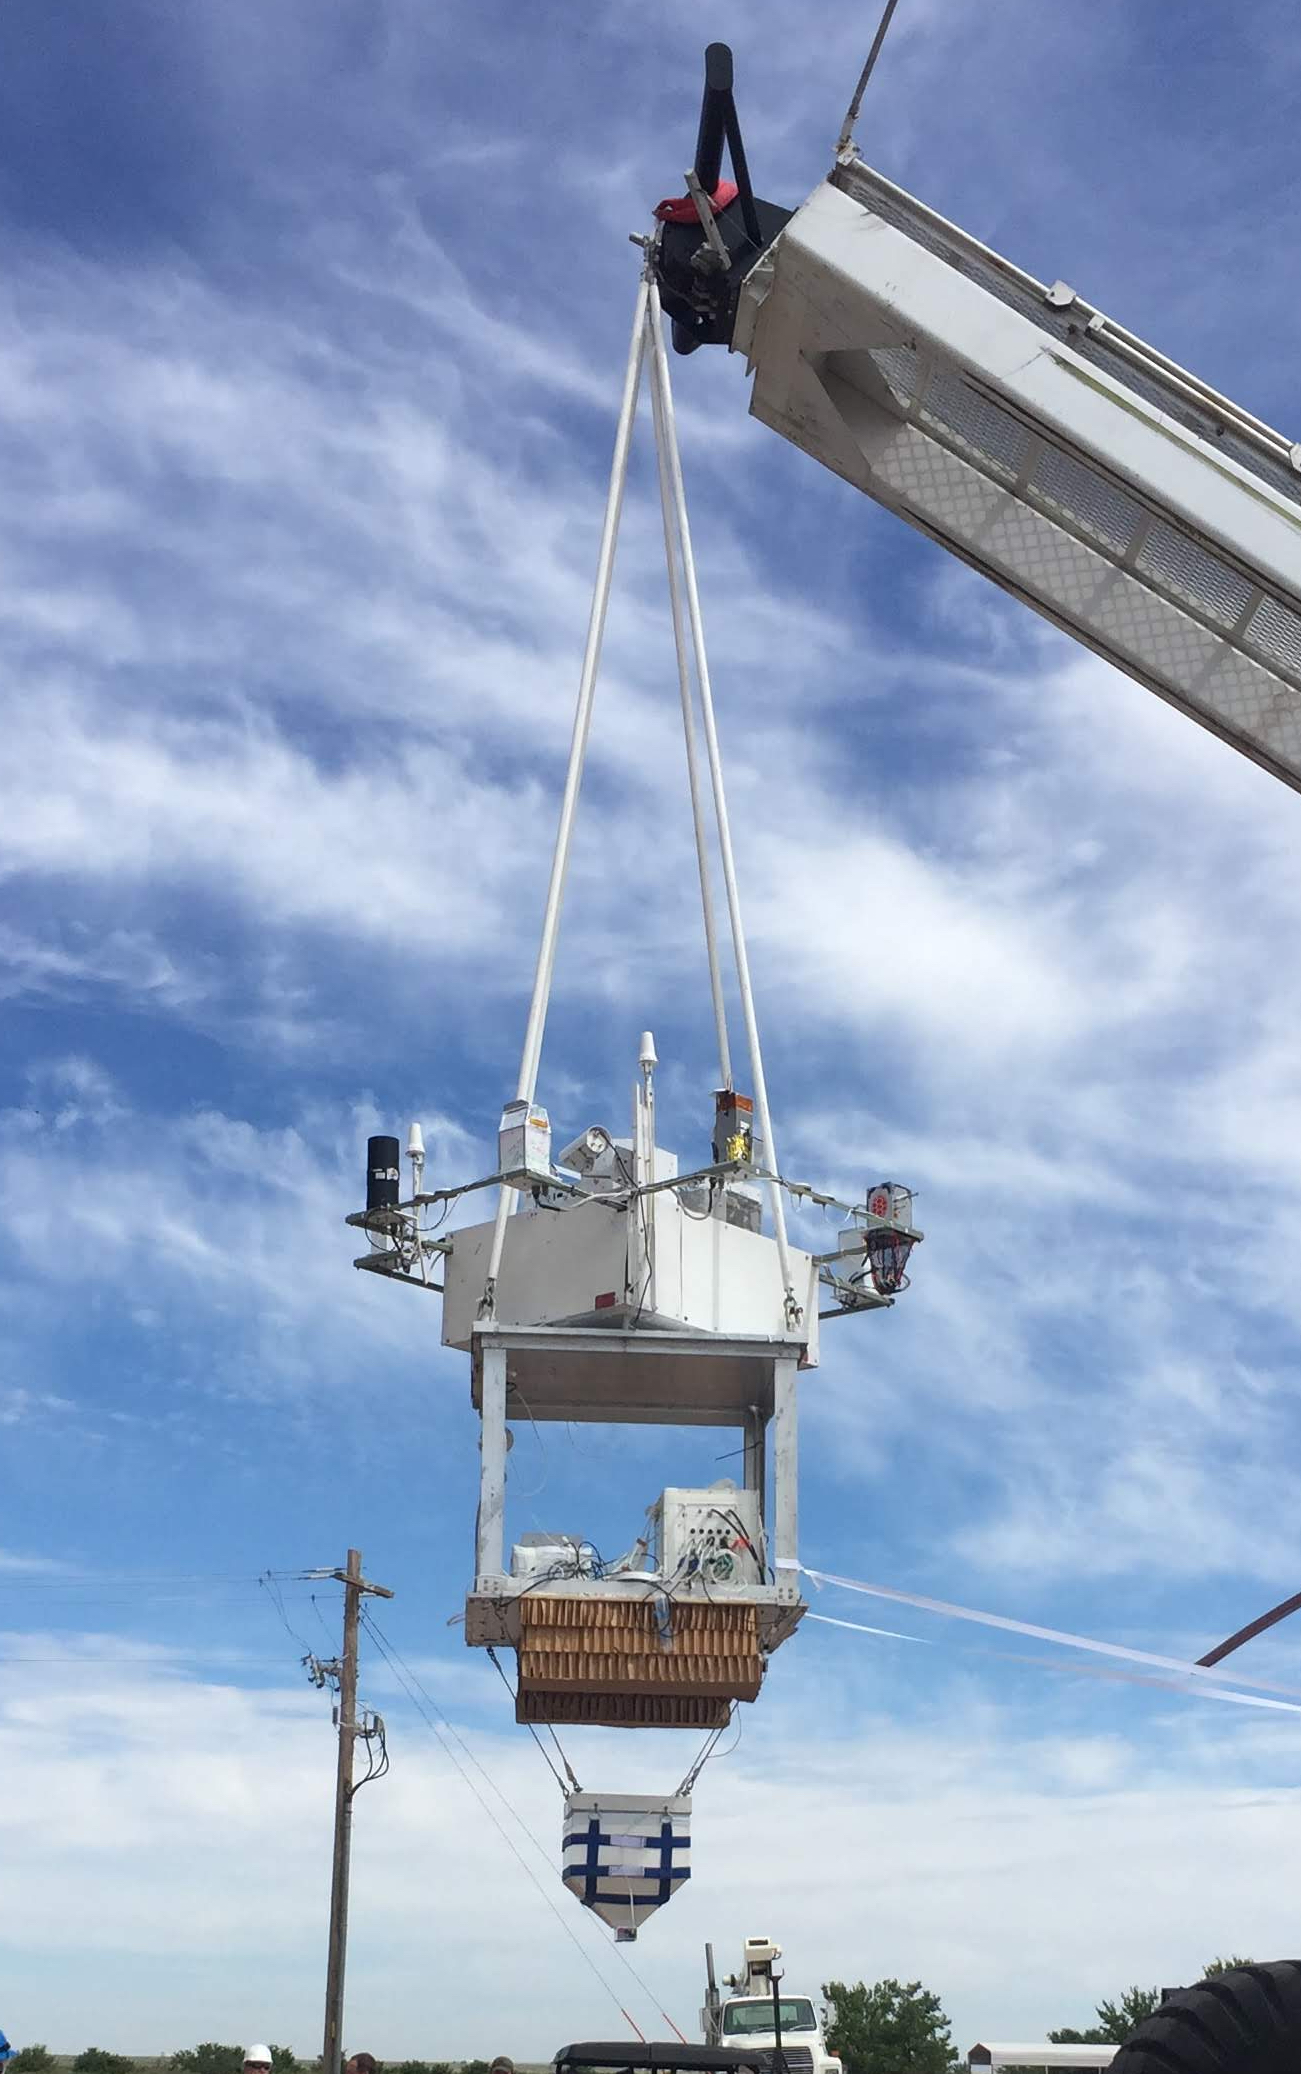
\includegraphics[width=50 mm, scale=0.5]{figures/gondola.jpg}
	\caption{Payload on the flightline}
	\label{fig:gondola}
	\end{center}
\end{figure}


%Intro (date, time, and information of general flight.  Weather conditions.  Official flight time.  Float start time and date, along with termination time and date.  Impact location.  Did it all go well?
Braving through inclement weather, SORA 2.0 took off early on September 4, 2018 at 14:03 UTC along with 12 student payloads.  From Ft. Sumner Municipal Airport, the payloads flew for approximately 9 hours.  The flight terminated at 1:31 UTC the same day and then landed shortly after at 2:11 UTC about 60 miles southwest of Mt Graham, Arizona.
%%%%%%%%%%%%%%%%%%%%%%%%%%%%%%%
\begin{table}[h!]
\centering
\caption{Flight information from NASA (SOURCE HERE)}
\label{flight_info}
\resizebox{\textwidth}{!}{%
\begin{tabular}{ll}
FLIGHT NUMBER:&688N \\
LAUNCH TIME:&09/04/2018 14:03:22 UTC \\
LAUNCH LOCATION:& 34.473162N 104.242232W \\
FLOAT START:&16:30:48 UTC \\
TERMINATION:&09/05/2018 01:31:23 UTC \\
FLOAT TIME:&09:00:35 \\
IMPACT:&02:11 UTC \\
IMPACT LOCATION:&32.44816666N 109.5093472W which is 60 miles SW of Mt Graham, Arizona 
\end{tabular}%
}
\end{table}

\begin{figure}[h!]
  \begin{center}
%    \begin{minipage}[c]{0.45\linewidth}
      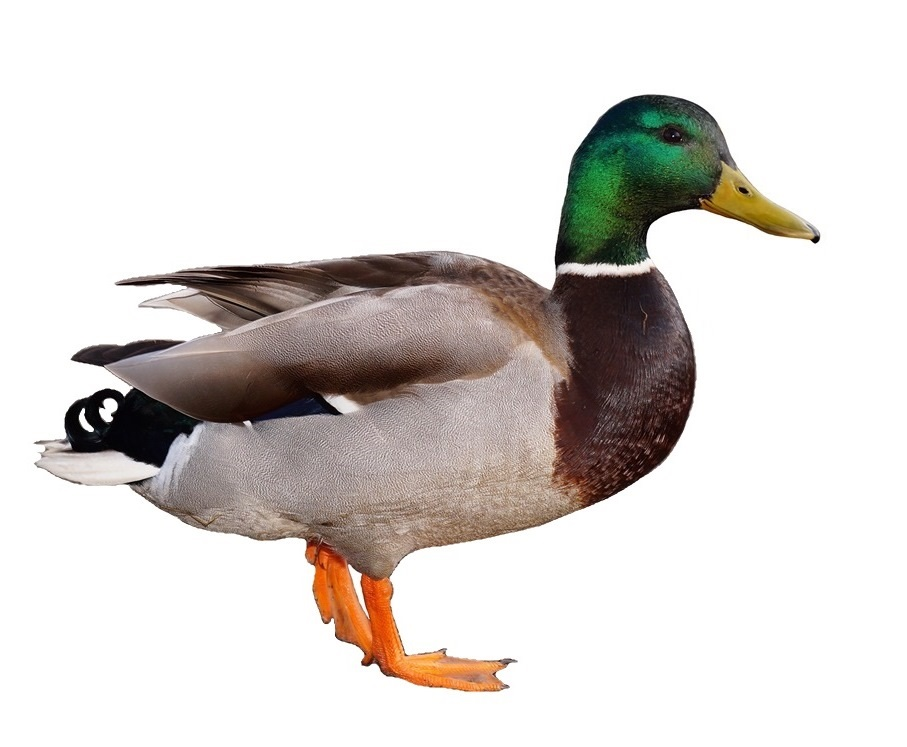
\includegraphics[width=\textwidth]{./figures/duck.jpg}
      \caption{just a duck}
      \label{fig:duck}
%    \end{minipage}
%    \hfill
%    \begin{minipage}[c]{0.49\linewidth}
%      \includegraphics[width=\textwidth]{./figures/name of figures.jpg}
%      \caption{}
%      \label{fig:}
%    \end{minipage}
  \end{center}
\end{figure}

%Mission statement and objectives:
%SORA 2.0 was a continuation of SORA~\cite{SORA} but this time seeking to . . .
SORA 2.0 was a continuation flight to further develop and build upon the first SORA flight \cite{SORA}.  SORA's first flight in 2017 collected valuable information, yet another mission was necessary to confirm and add to the findings of the first SORA flight.  Once again SORA attempted to collect extremophile bacteria and spores that may reside 36 to 41 kilometers in the upper atmosphere.  For the radiation portion of SORA 2.0, a MiniPIX particle detector in a custom built casing coupled with a boron-doped scintillator was also flown to further study the surrounding radiation and the possible effects on extremophiles.  
%%%%%%%%%%%%%%%%%%%%%%%%%%%%%%%%%%%%
%Past scientific questions:
% Are extremophiles present in the upper atmosphere at altitudes of 36 to 41 km?  If extremophiles are captured, can the SORA payload clean box container prevent sample contamination? Finally, can we collect data accurately enough to effectively study the effects of environmental radiation on extremophile organisms and spores.
 
%New scientific questions for SORA 2.0 from provisional application:
{\bf Scientific Questions}

The goals and objectives for SORA 2.0 are based on the following scientific questions: 
%
\begin{itemize}
	{\indentitem \item After confirming that microorganisms are present in the upper atmosphere in the first SORA mission, what extremophiles are present in the upper atmosphere at altitudes of 36 to 41 km?}
	{\indentitem \item If extremophiles are captured, can they be cultured and analyzed?}
	{\indentitem \item What methods are more effective at capturing bacteria for culturing?} 
	{\indentitem \item Finally, with a deeper understanding of the MiniPIX after the first SORA mission, can SORA 2.0 collect more data to study cosmic radiation that microoganisms and spores experience on a daily basis? Specifically, can SORA 2.0 obtain useful information about the biological effectiveness of this radiation on bacteria through parameters such as linear energy transfer and dose equivalent?}
\end{itemize}
%

%Did we complete our objectives?  If yes, what were they again (insert here briefly).  
%The main goals for SORA were to once again collect extremophile organisms that reside in the upper atmosphere, study the effects of surrounding radiation on these organisms in the stratosphere and gather data pertaining to the environmental conditions in which these organisms reside~\cite{SORA}.  

%From our provisional application:
%The main goals for SORA are to collect extremophile organisms that reside in the upper atmosphere, study the effects of surrounding radiation on these organisms in the stratosphere and gather data pertaining to the environmental conditions in which these organisms reside [1]. More specically, SORA has two sets of main objectives, along with four additional objectives.

%%%%%%%SORA 2.0 Objectives here.\\
% INSERT CITATIONS HERE SINCE WE ARE TAKING FROM OUR OWN APPLICATION

\begin{figure}[h!]
  \begin{center}
%    \begin{minipage}[c]{0.45\linewidth}
      
\includegraphics[width=\textwidth]{./figures/sam_meme.JPG}
      \caption{just a duck}
      \label{fig:duck}
%    \end{minipage}
%    \hfill
%    \begin{minipage}[c]{0.49\linewidth}
%      \includegraphics[width=\textwidth]{./figures/name of figures.jpg}
%      \caption{}
%      \label{fig:}
%    \end{minipage}
  \end{center}
\end{figure}
{\bf Primary Objectives:}
	\begin{enumerate}
	\item Using a refined astrobiology system, attempt to capture bacteria in the upper atmosphere at approximately \SIrange{30}{41}{\kilo\meter} of altitude.
%	
%
%	Need help from Fre'Etta and Jimish here...
	\item Conduct RNA analysis on samples
	\item Study the cosmic and background radiation that extromphiles may experience
	\end{enumerate}
%
%
{\bf Secondary Objectives:}
\begin{enumerate}
	\item Develop and simplify a radiation and payload flight control system.
%	\item Determine the polar angle of hits on the detector, compare them to payload orientation information and develop simulations to verify the results.
	\item Further testing of the astrobiology hardware in flight and the methodology for collection of microbes in extreme environments at high-altitude. 
	\item Improve pre and post-flight decontamination procedures.
%Engineering Objectives
	\item Implement a variable shutter time for the MiniPIX based on the flux of particles incident on the detector.
	\item Analyze the MiniPIX data in real time and downlink relevant radiation statistics.
	\item Implement a redundant data storage mechanism.
	\item Test an improved enclosure against impacts and harsh environments.
	\item Improve astrobiology collection mechanism.
\end{enumerate}
%%%%%%%%%%%%%%%%%%%%%%%%%%%%%%%%%%%%
\subsection{Hypothesis and Objectives}
\label{subsec:Hypothesis and Objectives}
\begin{enumerate}
%These are from provisional application:
%We need to review these, add more and remove some.
	\item Based on the collection results from previous HASP payloads we predict the concentration of cells at an altitude of 36 km will be less than 1000 cells per liter.
	\item Objective: Sample a minimum volumetric amount of air at target altitude for the duration of the float phase (approximately 15 to 18 hours).
	\item Based on control samples and testing before flight, we can compare our final flight results to previous applications.
	\item Objective: Quantify and characterize any contamination with our laboratory and payload disinfection procedures.
	\item Objective: Minimize the amount of external contamination before flight with thorough decontamination procedures.
	\item Based on measured results of dosage rates, the higher exposure to radiation may change the organism's cellular make-up.
	\item Objective: After capturing samples, analyze data and compare biological effects to similar genotypes found on Earth's surface.

\end{enumerate}


\begin{figure}[h!]
  \begin{center}
%    \begin{minipage}[c]{0.45\linewidth}
      
\includegraphics[width=\textwidth]{./figures/andrew_troll.jpg}
      \label{fig:duck}
%    \end{minipage}
%    \hfill
%    \begin{minipage}[c]{0.49\linewidth}
%      \includegraphics[width=\textwidth]{./figures/name of figures.jpg}
%      \caption{}
%      \label{fig:}
%    \end{minipage}
  \end{center}
\end{figure}
%Section: IntroAstrobiology
\subsection{Astrobiology}
\label{sec:Astrobiology-Background}
Extremophiles are microorganisms that thrive in physically and/or chemically extreme conditions in which most life cannot survive. These organisms and microbes have been found everywhere, from deep underwater volcano vents to buried ice lakes in Antarctica (1). 
%Antarctica [1] doesn't work, needs proper citation
Fungi and bacterial spores have also been found in the stratosphere. Today, the most common altitudes for organism and microbe collection in the atmosphere are in the range of approximately 10 km to 20 km above Earth’s surface. Very little data exists on microbiological samples captured in the stratosphere. 
%stratosphere [1] needs proper citation, NOT working in the compiler
Conditions at altitudes of 30km to 40km are extreme in temperature, pressure and radiation exposure. Arguably, each successful collection expedition, of at least 30 km into the upper atmosphere, provides information that can be useful in determining what life forms can exist inside and outside of Earth’s biosphere. Additionally, RNA analysis of the organisms and microbes can provide useful insight pertaining to their ability to survive in an environment with elevated levels of radiation.  

This year our experiment focused on designing a more compact collection apparatus and refining our sanitation procedures for preflight assembly, post flight disassembly, and RNA sequencing preparation. The samples we collected play an important role in expanding our knowledge about Earth’s biosphere. Future studies could produce meaningful contributions to the fields of gene therapy, RNA interface, and cosmic shielding; and provide valuable insight about how life can be distributed on Earth, and ultimately, through outer-space.


%Section: IntroRadiation
\subsection{Radiation}
\label{sec: Radiation Background}

Galactic cosmic rays (GCRs) are primary particles produced outside of the solar system \cite{GCRs}.
By colliding with other particles in Earth's atmosphere, GCRs can induce air showers consisting of secondary particles, which can be detected using sophisticated equipment.
These secondary particles can be measured, thus revealing information regarding the primary particle such as energy and direction. 
The density of all secondary particles \cite{Frank} is most dense in the troposphere at an altitude of about \SIrange{2}{3}{\kilo\meter}.
This is referred to as the atmospheric depth of the shower maximum $\chi _{max}$.
In terms of the SORA payload, this means that the bulk of the measured data during ascent and descent will 
be of secondary particles.
During float the particle distribution will have a larger contribution from primary particles.

Studying radiation dose is not only important for safety during spaceflight but is also important for safety during commerical airline flights.
Airplanes fly in the portion of the troposphere where air showers are at their peak in terms of particle density. As a consequence, passengers are exposed to relatively high doses of radiation.
At these altitudes, neutrons contribute significantly to the overall radiation composition<<FIND CITATION FOR THIS. ASK MALENA; SHE KNOWS>>

The MiniPIX \cite{silicon_sensor} is a silicon-based particle detector integrated with a Timepix \cite{timepix} chip. The device is a result of the Medipix Collaboration at CERN \cite{medipix}. 
When an energetic particle is incident upon the sensor, energy is deposited in the detector, and the resulting data is recorded.
For more detail regarding the functionality of the MiniPIX, refer to the previous flight report \cite{SORA}.
The MiniPIX's sensor can only detect charged particles, meaning it is unable to directly detect a neutron. However, through the use of a scintillator, the neutron can interact with the scintillator and produce a specific signature of charged particles which can be detected by the MiniPIX.
An example can be seen from Uher et al. \cite{Uher}, who use a lithium-based scintillator to detect neutrons using a silicon-based detector. The reaction is\ce{^6Li^+ + n -> ^3H+ \alpha (\SI{4.78}{\mega\eV})}.
This iteration of the SORA payload attemped a similar procedure to measure neutrons but through the use of a boron loaded plastic scintillator \cite{BoronScintillator}.
The scintillator had a 5\% boron loading and covered exactly half of the MiniPIX detector.
This particular scintillator was chosen due to its relatively larger reaction cross-section with neutrons.
The larger cross-section increases the probability that the neutron will produce particles which can then be deteted by the MiniPIX.

%Section: SORA Hardware Description
\section{SORA Payload Description}
\label{sec:Hardware}
%
\begin{figure}[h!]
	\begin{center}
		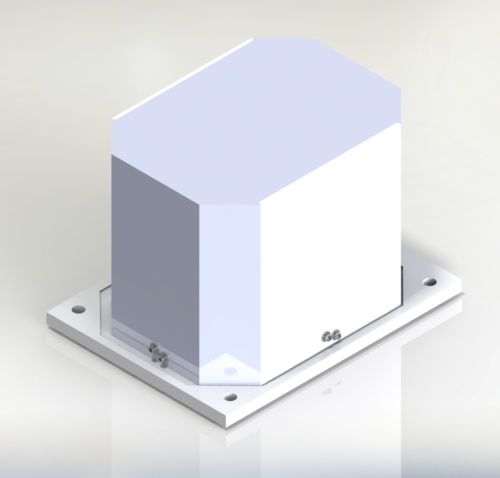
\includegraphics[width=50 mm, scale=0.7]{figures/payload_render.pdf}
		\caption{Payload Final Design}
		\label{fig:payload_render}
	\end{center}
\end{figure}
%
%
%
With the successful first flight of SORA in 2017, the UH team decided to use the same materials and methods to build SORA 2.0.  The design was optimized this year to use all the space available on the 2018 flight as shown on ~\ref{fig:payload_dim}.   The outer shell is KYDEX, a composite made of PVC and acrylic. KYDEX	 was initially chosen due to its properties.  It is hydrophobic, UV resistant, and can withstand a wide range of conditions.  It has a tensile strength of 6,100 PSI (INSERT MCMASTER SOURCE) and an impact strength of 15.00 ft.-lbs./in (SOURCE AND FIX THE UNITS).  The bolts used on the payload mainly were iron bolts with a weather-resistant coating.   Brackets and other wall-mounting parts were nickel plated off-the-shelf parts.
\begin{figure}[h!]
	\begin{center}
		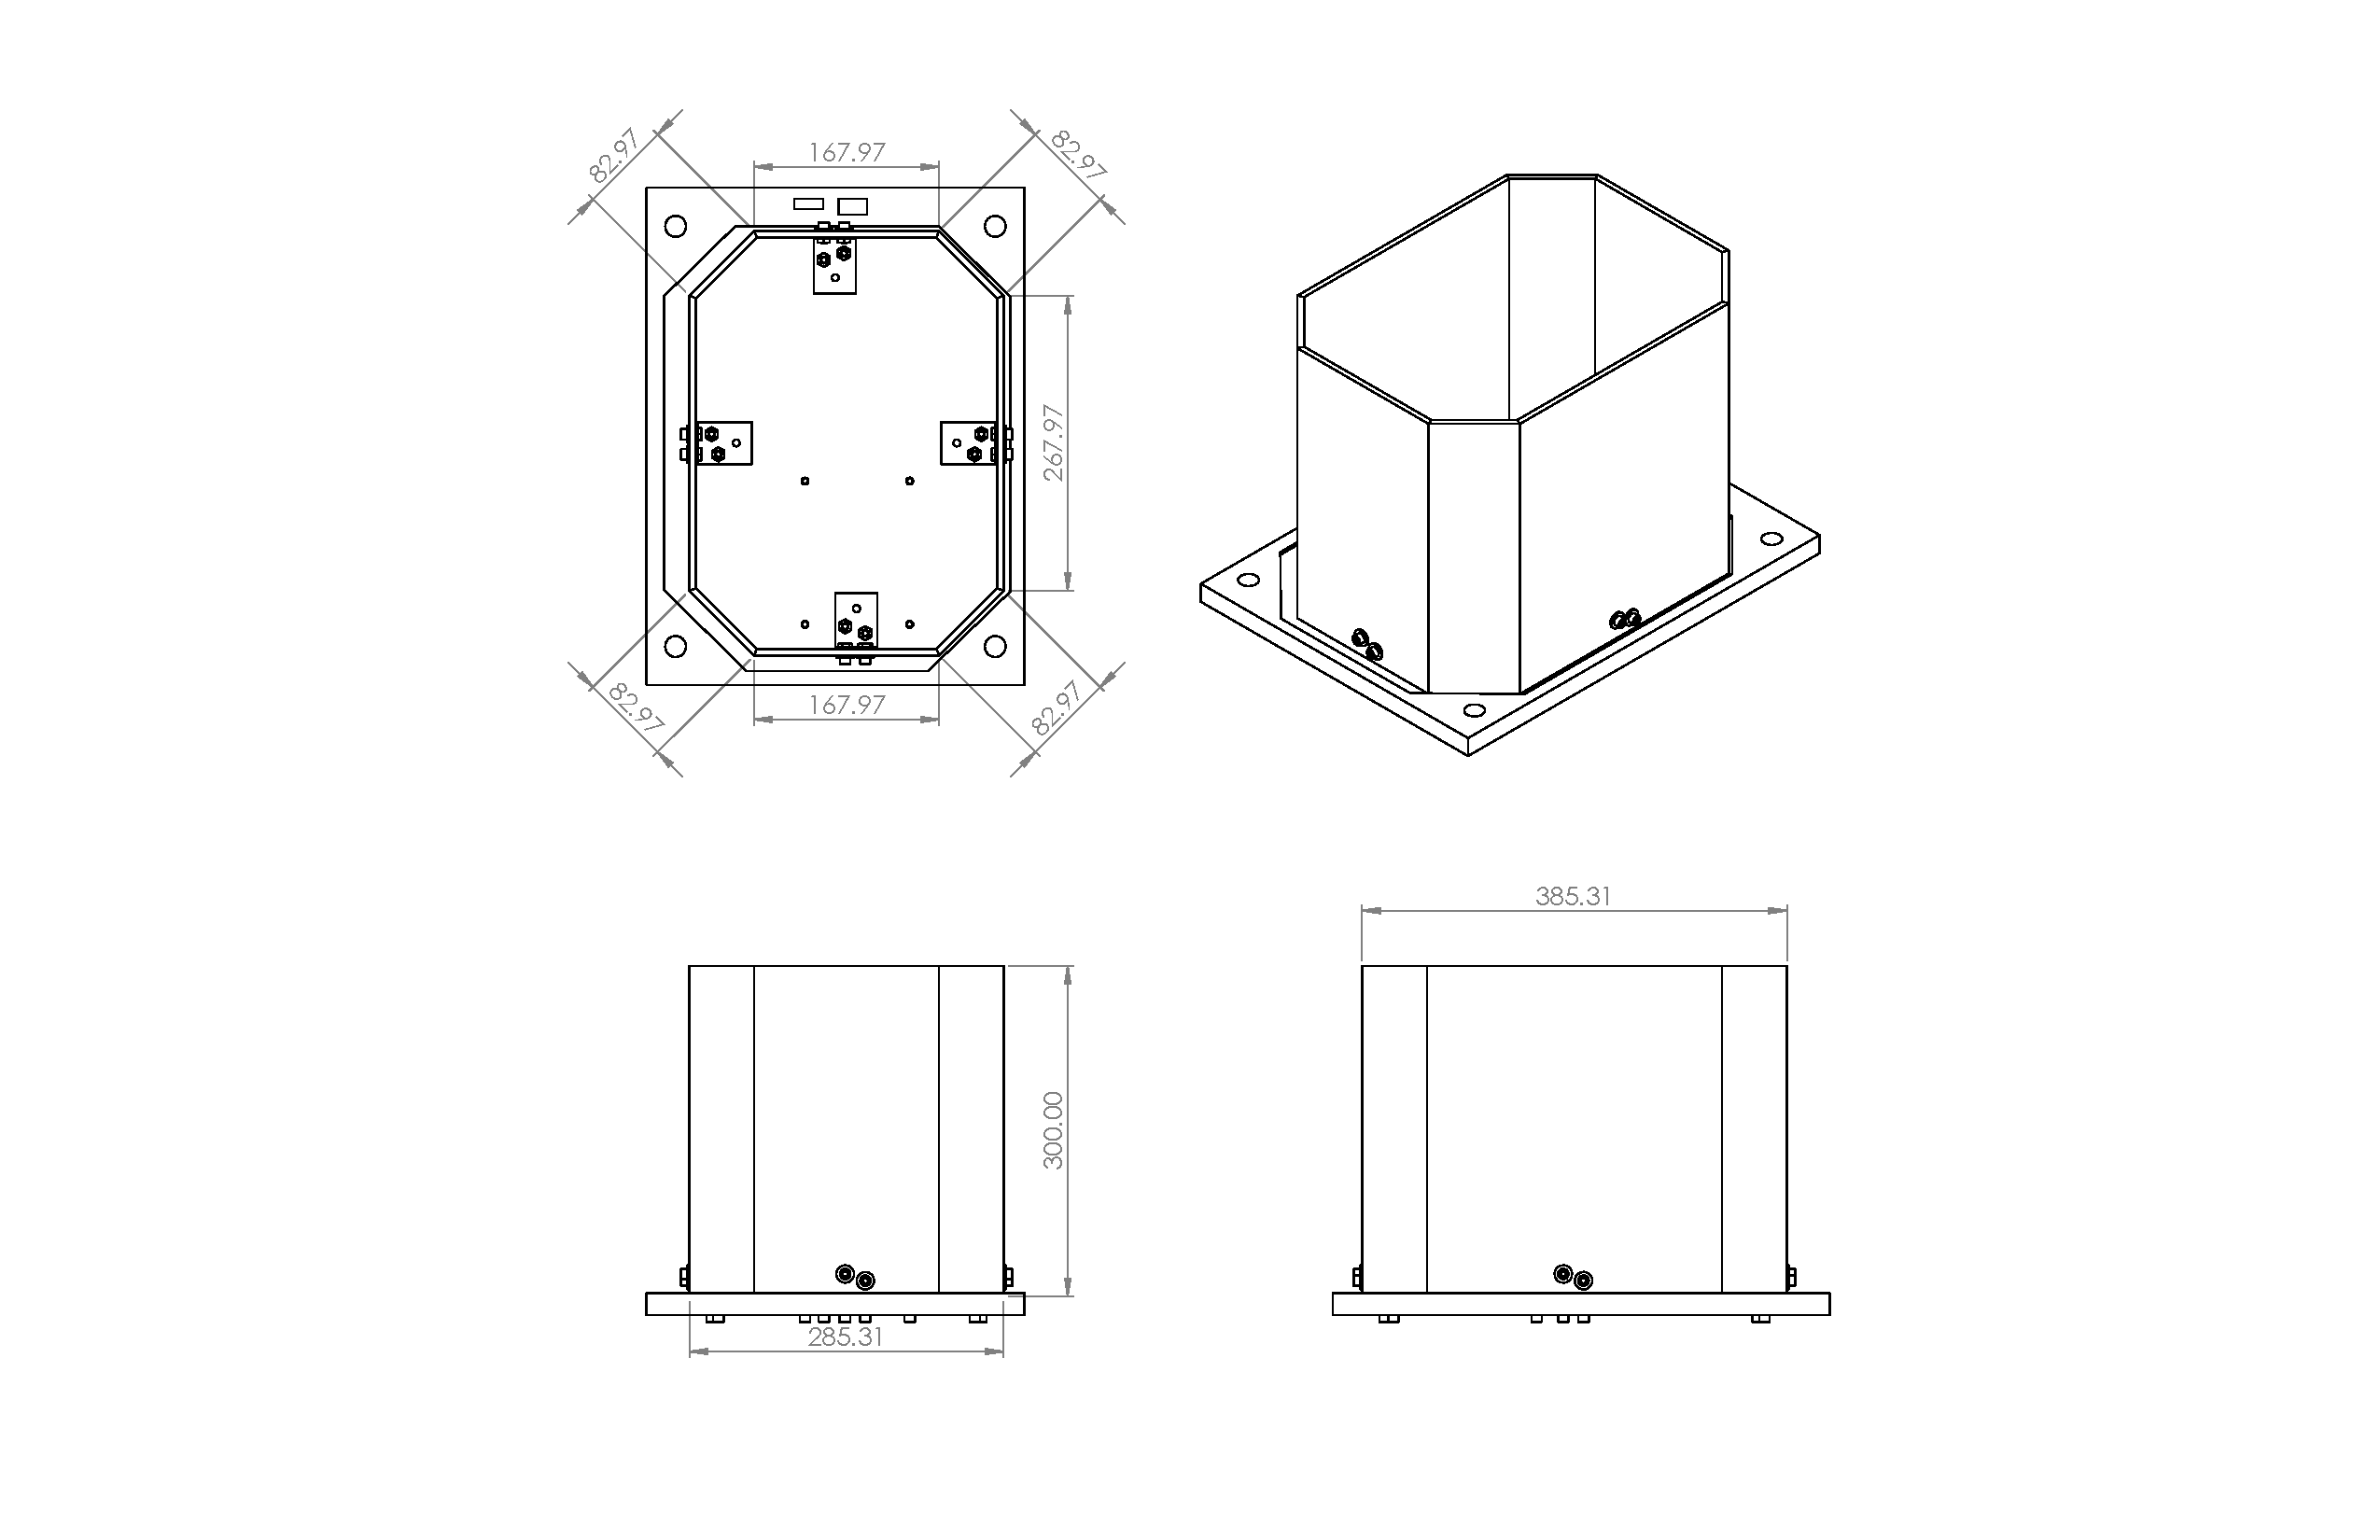
\includegraphics[width=50 mm, scale=0.7]{figures/payload_dimensions.PDF}
		\caption{Payload Dimensions}
		\label{fig:payload_dim}
	\end{center}
\end{figure}
%%%%%call out a figure.       ~\ref{fig:}
%Subsections:
%Talk about general design of each component or payload part.  Go into detail about choice of materials, placement, and reasoning for the success of the mission.  Also, try to include either real photos, CAD designs or any other relevant graphic.  
%\subsection{MiniPIX}
%MiniPIX
%\subsection{Flight Computer and Sensors}
%Flight Computer and Sensors (include the electric schematics)
%\subsection{Astrobiology}
%Astrobiology (lots of CAD designs)
%\subsection{Payload Structure and Outer Shell}
%Outer Shell (CAD designs and choice of materials)
%Notes:
%Outer material is Kydex from McMasterCarr
%Part PVC and part acrylic
%Manufacturer Specs:
%	https://www.mcmaster.com/acrylic/pvc
%	hydrophobic
%	UV resistant - no sun deterioration
%	3/16 inch thick
%	Color - white
%	Temperature range from -40 F to 150 F
%	Tensile Strength of 6,100 psi
%	Impact strength 15.00 ft.-lbs./in 
%	UL 94V0
%Commonly used for vehicle interiors and equipment housings, this material maintains its shape after heating and forming. It is also known as Kydex. These sheets resist corrosive chemicals and cleaning solutions. One side is smooth; the other side is coarse to mask scratches, scuffs, and fingerprints.
%
%Coated iron bolts, standard size for heavy mounting options
%Nickle plated L-brackets and brackets for wall mounting
%Machine cut to specifications (will include a figure here with all the dimensions)
%\begin{figure}[h!]
%	\begin{center}
%		\includegraphics[width=\textwidth]{figures/[figure name here]}
%		\caption{Payload Final Design}
%		\label{fig:payload_design}
%	\end{center}
%\end{figure}
%
%\begin{figure}[h!]
%	\begin{center}
%		\includegraphics[width=\textwidth]{figures/[figure name here]}
%		\caption{Picture of payload mounted onto gondola}
%		\label{fig:payload_gondola}
%	\end{center}
%\end{figure}

\input{Design_RESU.tex}
\subsection{Astrobiology System Design}
\label{sec:Astrobiology Design}
The collection assembly was designed as a two-compartment structure, with one experimental collection and one control container, one pump, and two solenoids. The clean box and containers were machined from impact-resistant UHMWPE (1). 
%UHMWPE [1] need proper fixing, the citation doesn't work in the compiler
The control container was connected to a solenoid that remained closed until post-flight sanitization procedures were performed. The experimental sample collection container was connected to a vacuum pump located outside of the clean box structure. Once float altitude was reached, the solenoid connected to the experimental sample collection container was opened and the pump was powered on; allowing air to flow to the collection container. Each container held approximately 2 mL of a 15 \% sterile glycerol solution. A 316 Stainless Steel 1/4" NPT Vent to Atmosphere Vitron Seal Valve was embedded in each of the compartments, to accommodate for the pressure changes that occurred with the variations in altitude over the course of the flight. The left side of Figure ??? displays the clean box structure, showing the bottles inside and the lids with the openings for the sample and exhaust tubing, while the right side of Figure 4 shows the 3D rendering of the sampling pump.
\subsection{Radiation Monitoring System Design}
\label{sec:Radiation Design}
The Raspberry Pi has proven to operate at float altitudes both from the previous SORA flight and other HASP payloads from previous years and as such was chosen again to host the control and analysis software. Similarly to the SORA 1.0 flight, both TimePIX devices were interfaced with the RPI via USB and controlled via the pypixet library developed at CERN by (Daniel Turcek?). The major difference for the 2018 SORA flight is that the software was redesigned to support an arbitrary number of TimePIX devices to record data at the same time. This means that multiple TimePIX detector experiments could be run concurrently without adding another control system. Another major difference is that the detectors could be configured directly from the serial uplink and collected data could be downlinked in real time. This allowed data from the detector to be analyzed and plotted in real time by the members of our team.

The control and analysis software was written entirely in Python and operated directly on top of the default Raspbian image. Because the pypixet software blocks when exposing the detector for collection, both detectors had to collect data in their own threads to allow the main thread to process uplink commands and control other systems. Data from each of these threads was then placed onto a queue where the main thread could periodically check if there was data ready to be processed. When a frame from one of the detectors was ready to be processed the main thread performed the analysis and then downlinked the results. Consequently, downlink speed was directly tied to shutter speed. An overview of the software design is shown in Figure (INSERT REFERENCE HERE)
%\ref{softwaredesign}.THIS WAS MOVED HERE SINCE IT WAS AFFECTING THE COMPILER - NEEDS TO BE PROPERLY DEFINED

\begin{figure}[h!]
	\begin{center}
	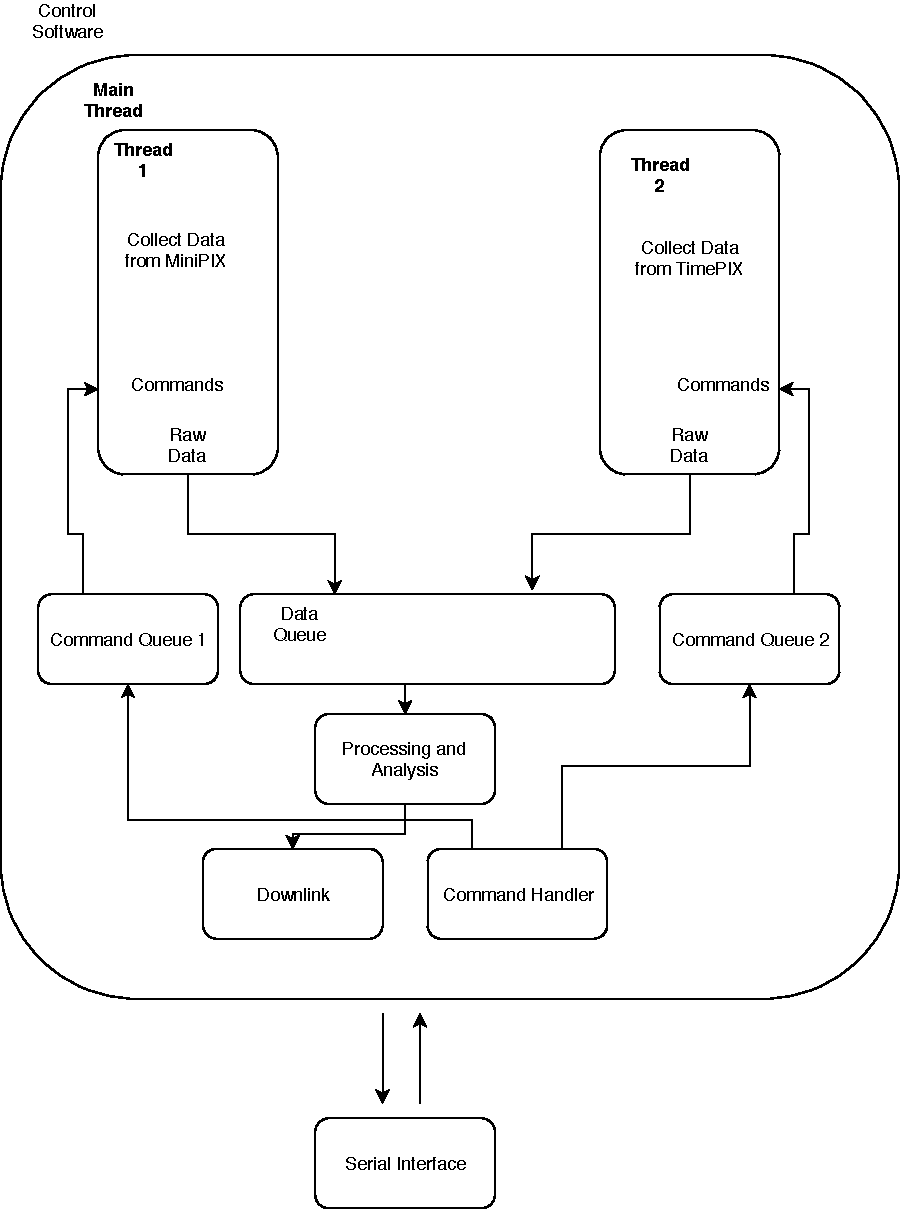
\includegraphics[width=0.5\textwidth]{figures/SoftwareDesign.pdf}
	\caption{Software design for the radiation control systems.}
	\label{fig:softwaredesign}
	\end{center}
\end{figure}
\clearpage
 
By and large the MiniPIX, and TimePIX detectors have proven to be robust and resilient towards large thermal fluctuations. However, during the course of integration testing in Palestine a failure was observed. During the cold cycle of the test a slow but steadily increasing number of counts was observed that is anomalous to what one would expect near the earths surface. The expected number of counts per second should've been close to 3 but the downlinked data was reporting values of over 300 as shown in Figure (INSERT FIGURE REFERENCE HERE)
%\ref{integrationtemps}.  THIS WAS MOVED HERE SINCE IT WAS AFFECTING THE COMPILER - NEEDS TO BE PROPERLY DEFINED
A correlation analysis was performed and showed that there was no direct correlation between device counts and temperature. Additionally, this behavior was not observed on an identical detector used during the 2017 SORA flight. 

After consulting with some of the members of the TimePIX collaboration at the University of Houston and NASA we were informed that they were unable to determine a concrete reason for the failure but did provide a couple of possible explanations. The first, but most unlikely cause is that of a single event upset in the device causing the detector threshold to be lowered. TimePIX devices deployed on the International Space Station often experience this kind of behavior and consequently reload their configurations every few frames to prevent it. This is an exceedingly unlikely possibility in our case however, given the low levels of high energy particles near the earths surface. Another possibility is that the cold caused a partial failure in the power supply and the RPI was unable to provide enough power to the detector. This explanation is somewhat more likely, but because this kind of failure was never observed again it is difficult to say definitively what the cause was.

\begin{figure}[h!]
	\begin{center}
	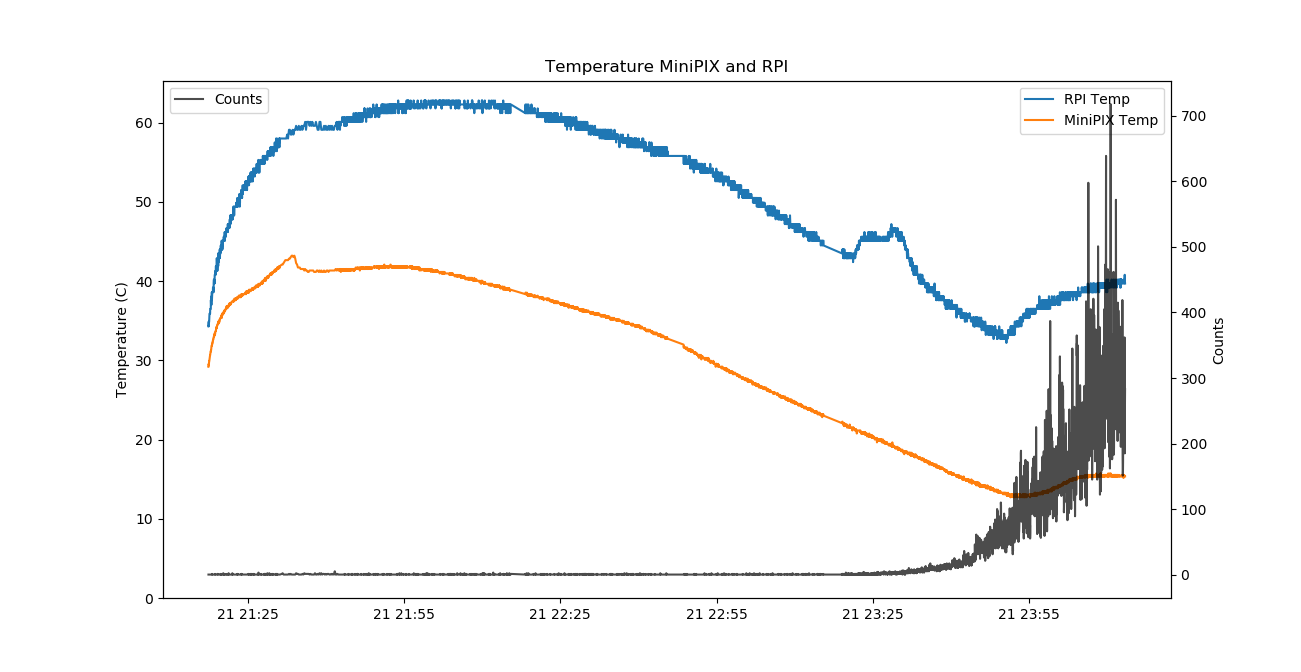
\includegraphics[width=\textwidth]{figures/tempsandcountsvtime.png}
	\caption{Temperature of flight computer and detector and counts.}
	\label{integrationtemps}
	\end{center}
\end{figure}

\subsection{Telemetry}
\label{sec:Telemetry}

All telemetry was handled via the RPi. The DB9 interface from the HASP Large Payload plate was converted to a 
RS-232 female plug. A Male RS 232 to Male USB was used to connect it to a USB port of the RPi. 
The downlink data packets were written to describe the radiation data. 
The uplink commands were sent to the RPi which delegated the work either to itself or the Arduino which 
was connected to the RPi via USB.

\subsubsection{Uplink}
\label{sec:Uplink} 
Uplink commands were used to start, end, and change parameters within our payload over the course of flight. 
Table \ref{tab:All-Commands} list the uplink commands, thier functions and a brief description of what they did. 

\subsubsection{Downlink}
\label{sec:Downlink}
Downlink data was written to describe the data being read from the MiniPix detector. 

\begin{table}[h!]
\centering
\caption{Table of All Uplink Commands Used During Flight}
\label{tab:All-Commands}
\bigskip
\begin{tabular}{c|c|c|c}
\hline
\hline
\multicolumn{1}{c|}{\bfseries Command} & \multicolumn{1}{c|}{\bfseries Byte 1} &  \multicolumn{1}{c|}{\bfseries Byte 2} & \multicolumn{1}{c}{\bfseries Expected Current Consumption} \\
\hline
	Start Acquisition  		& 0x01	& -	 				& \SI{0.47}{\ampere}    \\ \hline
	End Acquistion 			& 0x02	& -	 				& \SI{0.29}{\ampere}    \\ \hline
	Change Shutter Rate 	& 0x03 	& 0x01 to 0xFF *	& nominal A 		\\ \hline
	Change Acquisition Mode	& 0x04	& 0x01 or 0x02 **	& nominal A		\\ \hline
	Astrobiology System On	& 0x05	& -					& spike			\\ \hline
	Astrobiology System Off	& 0x06	& -					& nominal		\\ \hline
\end{tabular}
\medskip
\end{table}

Below is a sample of real data packets recieved during flight. 

\lstset{basicstyle=\small, numbers=left, xleftmargin=2em, frame=tb, label = Downlinks, framexleftmargin=1.5em}
\begin{lstlisting}[caption = Sample of downlinked data packets ID: 15667 - 15670.]
...
some samples here
...
\end{lstlisting}


%Section: Methods
%\newpage
\section{Methods}
\label{sec:Methods}

%\begin{figure}[!htb]
%\begin{center}
%
\includegraphics[width=0.5\textwidth]{./Figures/Test.jpg}
%\caption{This is a test figure.}
%\label{fig:Test} 
%\end{center}
%\end{figure}
\input{Methods_RESU.tex}
%\begin{Document}
\subsection{Astrobiology Methods}
\label{sec:Astrobiology Methods}
 The clean box, the collection containers, and the tubing used to connect the components were all autoclaved for sterilization. A 70\% ethanol solution was circulated through the pump to sterilize the internals. Everything used to assemble the system was then sprayed down with the ethanol solution before being placed inside a SterilGARD e3 Class II Biological Safety Cabinet. The 15\% glycerol solution was pipetted into each container, the lids were sealed with epoxy, and tubing was inserted and epoxied into the holes in the container lid. Each lid had two holes, one that led to the inside of the clean box to allow for pressure to be released from inside the container and out-gassed through the valves embedded in the clean box, while the other hole passed through the clean box lid to allow the tubing to connect to the pump, or pass through the solenoid only in the case of the control tubing. The clean box was apportioned to keep the experimental and control containers completely isolated from one another. Each container had their own pressure relief valve leading from their individual compartment within the clean box to the outside of the clean box. The lid to the clean box was sealed with epoxy and bolted closed, the tube from the control container was clamped by the dedicated control solenoid, while the tube from the experimental container was passed through the other solenoid and connected to the out-gassing nodule on the pump. The two holes in the clean box lid were sealed with epoxy and gasket maker to secure the tubing in place. The tube connected to the intake nodule on the pump was stabilized through an opening in the payload wall. The solenoid clamping the tubing to the experimental container remained closed until float conditions were achieved. Fluropore membrane filters (\SI{13}{\milli\meter}; \SI{22}{\micro\meter}) were used to collect control samples in the labs where work was conducted and on the inside walls of the payload. 
 
 The payload was successfully retrieved on September 6, 2018. The intact payload was shipped to the University of Houston and received on September 12, 2018. The clean box and background samples were removed and placed in cold storage at \SI{-20}{\celsius}.

 All equipment used in the filtration process was either autoclaved or taken from previously unopened sanitized packaging. The autoclaved, pre-sanitized items and the clean box were washed in a 70\% ethanol solution before they were placed inside the Biological Safety Cabinet previously mentioned. 
 The payload was successfully retrieved on September 6, 2018. The intact payload was shipped to the University of Houston and received on September 12, 2018. The clean box and background samples were removed and placed in cold storage at \SI{-20}{\celsius}. All equipment used in the filtration process was either autoclaved or taken from previously unopened sanitized packaging. The autoclaved, pre-sanitized items and the clean box were washed in a 70\% ethanol solution before they were placed inside the Biological Safety Cabinet previously mentioned. 
 
The control sample collection solution was vacuum filtered through a Fluropore membrane filter (\SI{13}{\milli\meter}; \SI{22}{\micro\meter}) to collect specimens on the filter surface. The experimental sample collection container was thoroughly swabbed with a Fluropore membrane filter as the glycerol coated the inside of the container and the full sample could not be pipetted out of the container to pass through the vacuum and onto the filter. All filters were processed using the DNeasy PowerWater Kit by QIAGEN \cite{PowerWaterKit} in preparation for 16S ribosomal RNA sequencing.   









%\end{Document}

\subsection{Cosmic Radiation Methods}
\label{sec:Rad-Methods}

\begin{figure}[H]
	\begin{center}
	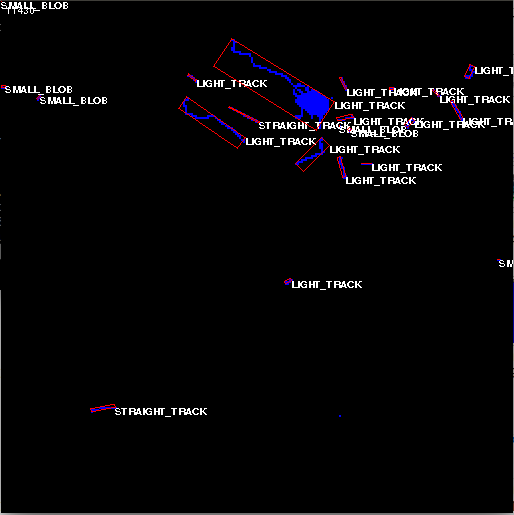
\includegraphics[width=0.6\textwidth]{figures/clustering.png}
	\caption{Bounding boxes calculated for a frame of flight data.}
	\label{clusterframe}
	\end{center}
\end{figure}

The output format of TimePIX devices provides a great deal of flexibility in terms of data analysis. The data can provide both a simple absorbed dose from ionizing radiation as well as insight into more detailed dosimetric endpoints like dose equivalent. Additionally a clustering procedure can be performed to analyze individual particle interactions in the detector based on their morphological properties.

 Since energy deposition can be determined on a per pixel basis, absorbed energy is calculated via a simple summation across all pixels in a frame of data after applying a standard calibration procedure \cite{mpjakubek}. With knowledge of the mass of the detector volume you can then calculate a dose by dividing the deposited energy by the detector mass. Thus a simple dose in silicon is calculated as

\[D_{Si} = \frac{E}{M_{d}}\]

To analyze the data on a per track basis first, a clustering procedure has to be performed to separate the data in a frame into individual tracks. This can be accomplished by applying a simple algorithm used in image processing called Flood-Fill; whereby contiguous nonzero pixels are recursively filled and grouped together into clusters. Then, after calculating a minimum area bounding box and linear least squares fit a track length is calculated by determining where the least square fit line intersects with the bounding box. Additionally, an azimuth angle can be determined relative to the detector orientation and a density can be calculated by dividing the number of pixels in a cluster by the area of the bounding box. A simple visual example of these calculations is shown in Figure \ref{track_analysis} and a visualization of the bounding boxes calculated for a frame of data is shown in Figure \ref{clusterframe}

\begin{figure}[H]
	\begin{center}
	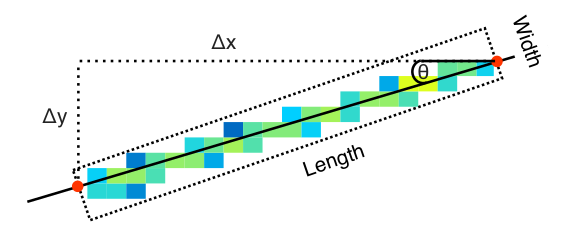
\includegraphics[width=0.8\textwidth]{figures/density.png}
	\caption{Track parameter calculation.\cite{stuartthesis}}
	\label{track_analysis}
	\end{center}
\end{figure}

Given the track length calculated from the fit line and the bounding box, a three-dimensional track through the detector by using simple trigonometry. Given the sensor thickness $T$ and the projected track length $L_{p}$ the length of the track through the detector $L$ can be calculated by

\[L = \sqrt{L_{p}^{2} + T^{2}} \]

With a true track length calculated one can then calculate the linear energy transfer ($LET$) of a track by dividing the total energy deposited in a cluster $E$ by the track length $L$.

\[LET_{Si} = \frac{E}{L}\]





Another standard technique used when analyzing TimePIX data is sorting clusters in the data based on their morphological characteristics. After clustering, additional processing is applied to calculate individual track parameters. These parameters can then be placed into a simple sorting algorithm that assigns them labels based roughly on their characteristics. The idea behind this morphological analysis is that information regarding the origin of the particle that made the track can be elucidated on the principle that similar types of particles will create similar shaped tracks in the detector. Based on a tracks density, pixel count, inner pixel count and ratio between the bounding box's length and width a track is sorted as either a small blob, medium blob, heavy blob, light track, straight track or heavy track. The specifics of the algorithm are defined in Figure \ref{stuart_algo}.

\begin{figure}[H]
	\begin{center}
	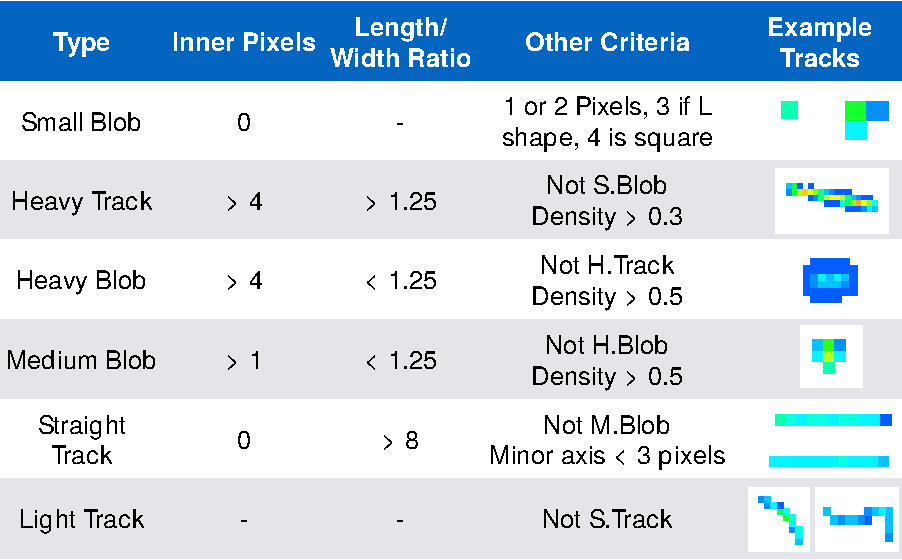
\includegraphics[width=0.65\textwidth]{figures/stuartgraphic.pdf}
	\caption{Track morphology algorithm.\cite{stuartalgo}}
	\label{stuart_algo}
	\end{center}
\end{figure}

While the track morphology does not provide a hard and fast classification a rough idea of the origin of a track in a mixed radiation field can be determined. Possible origins of track morphology are shown in \ref{track_morphology}.

\begin{figure}[H]
	\begin{center}
	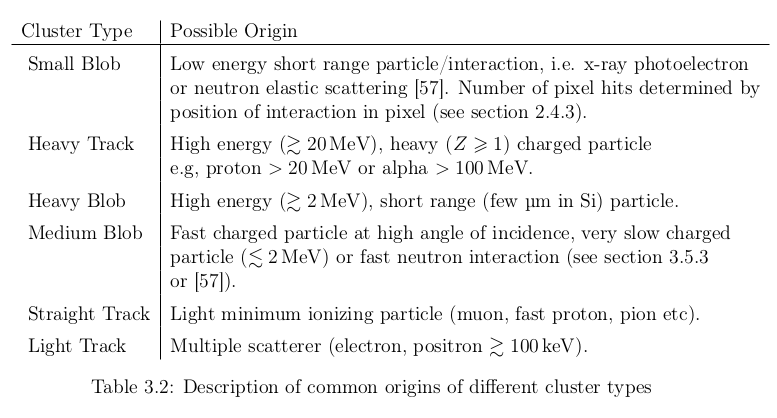
\includegraphics[width=0.8\textwidth]{figures/cluster_types.png}
	\caption{Possible physical origins of cluster morphology.\cite{stuartthesis}}
	\label{track_morphology}
	\end{center}
\end{figure}


%Results and Analysis
%Section: Flight Conditions and Environmental Data
\section{Results}
\label{sec:Results}
 %RESU first
\subsection{Cosmic Radiation Results}
\label{sec:Cosmic-Radiation-Results}

During the duration of the flight, a total of 16376 frames were collected and recovered successfully from the payload. Shown in Figure \ref{tracks} are a sample of tracks collected at float. The image in the upper left likely shows an interaction from a heavy ion while the rest of the tracks show a sampling of light and straight tracks. 


\begin{figure}[H]
	\begin{center}
	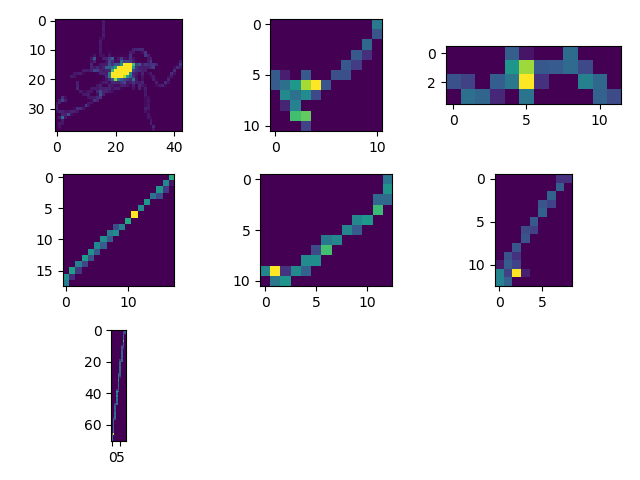
\includegraphics[width=0.75\textwidth]{figures/tracks.png}
	\caption{Tracks collected at float.}
	\label{tracks}
	\end{center}
\end{figure}

Shown in Figure \ref{let} (a) is the LET distribution for the entire population of tracks collected at float while \ref{let} (b) shows the LET distribution split up by track classification.

\begin{figure}[H]
\hfill
\subfigure[LET histogram from data collected during the duration of the flight.]{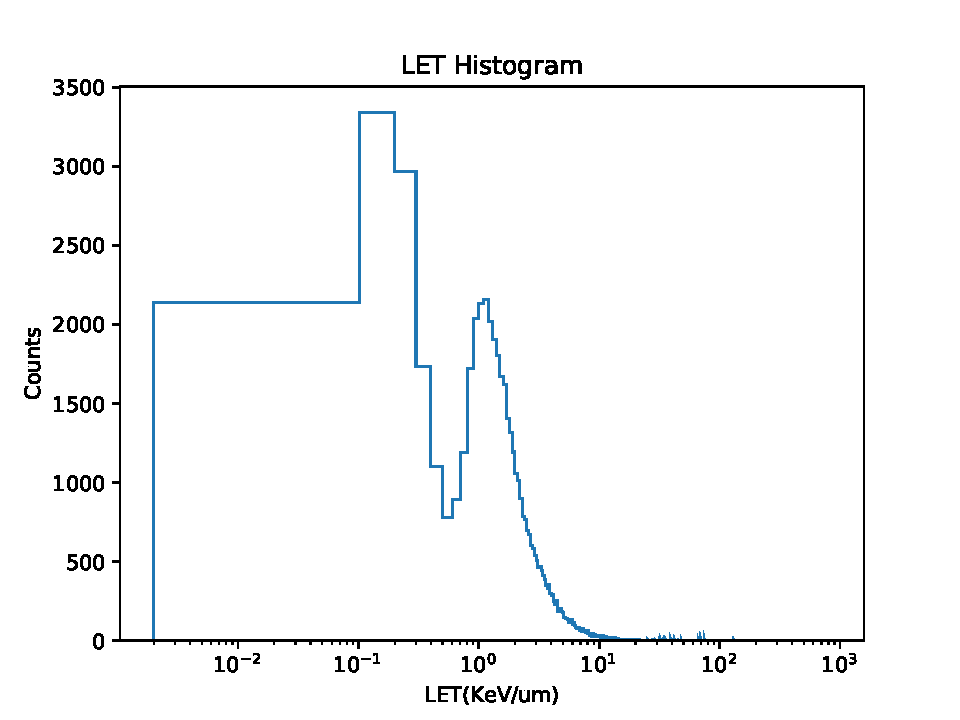
\includegraphics[width=8cm]{figures/LETSpectra2018.pdf}}
\hfill
\subfigure[LET histogram from each cluster type.]{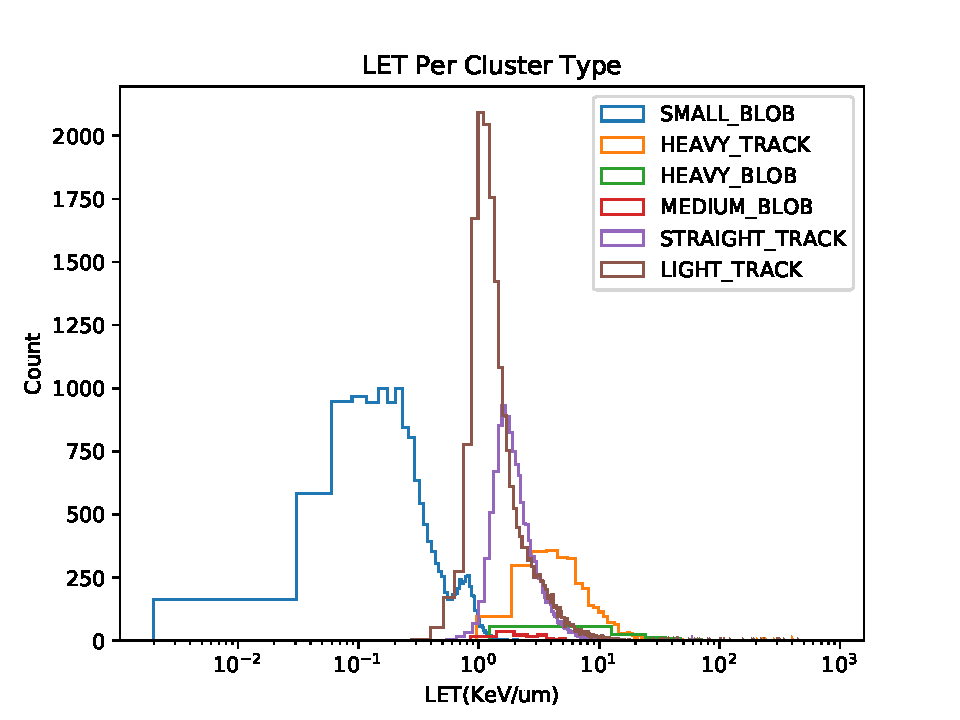
\includegraphics[width=8cm]{figures/LETSpectraPerCluster2018.pdf}}
\hfill
\caption{LET distributions data from Flight}
\label{let}
\end{figure}

Shown in Figure \ref{counts} is a comparison of the count rate for the SORA 2017 and 2018 flight. The shape of the data is nearly identical however one can observe that the 2018 flight has a higher variability and is slightly less homogeneous when compared to the 2017 data. The overall variability is due to a faster frame rate and the period of decreased variability that occurs just after the peak is due to a test of the ability to dynamically modify the frame rate via uplink commands. Another significant feature of the data is that the 2018 flight appears to be shifted upwards by approximately two counts per second when compared to the 2017 data. This would seem to suggest a higher flux during the 2018 flight.
\begin{figure}[H]
\hfill
\subfigure[Counts from data collected during the 2017 flight.]{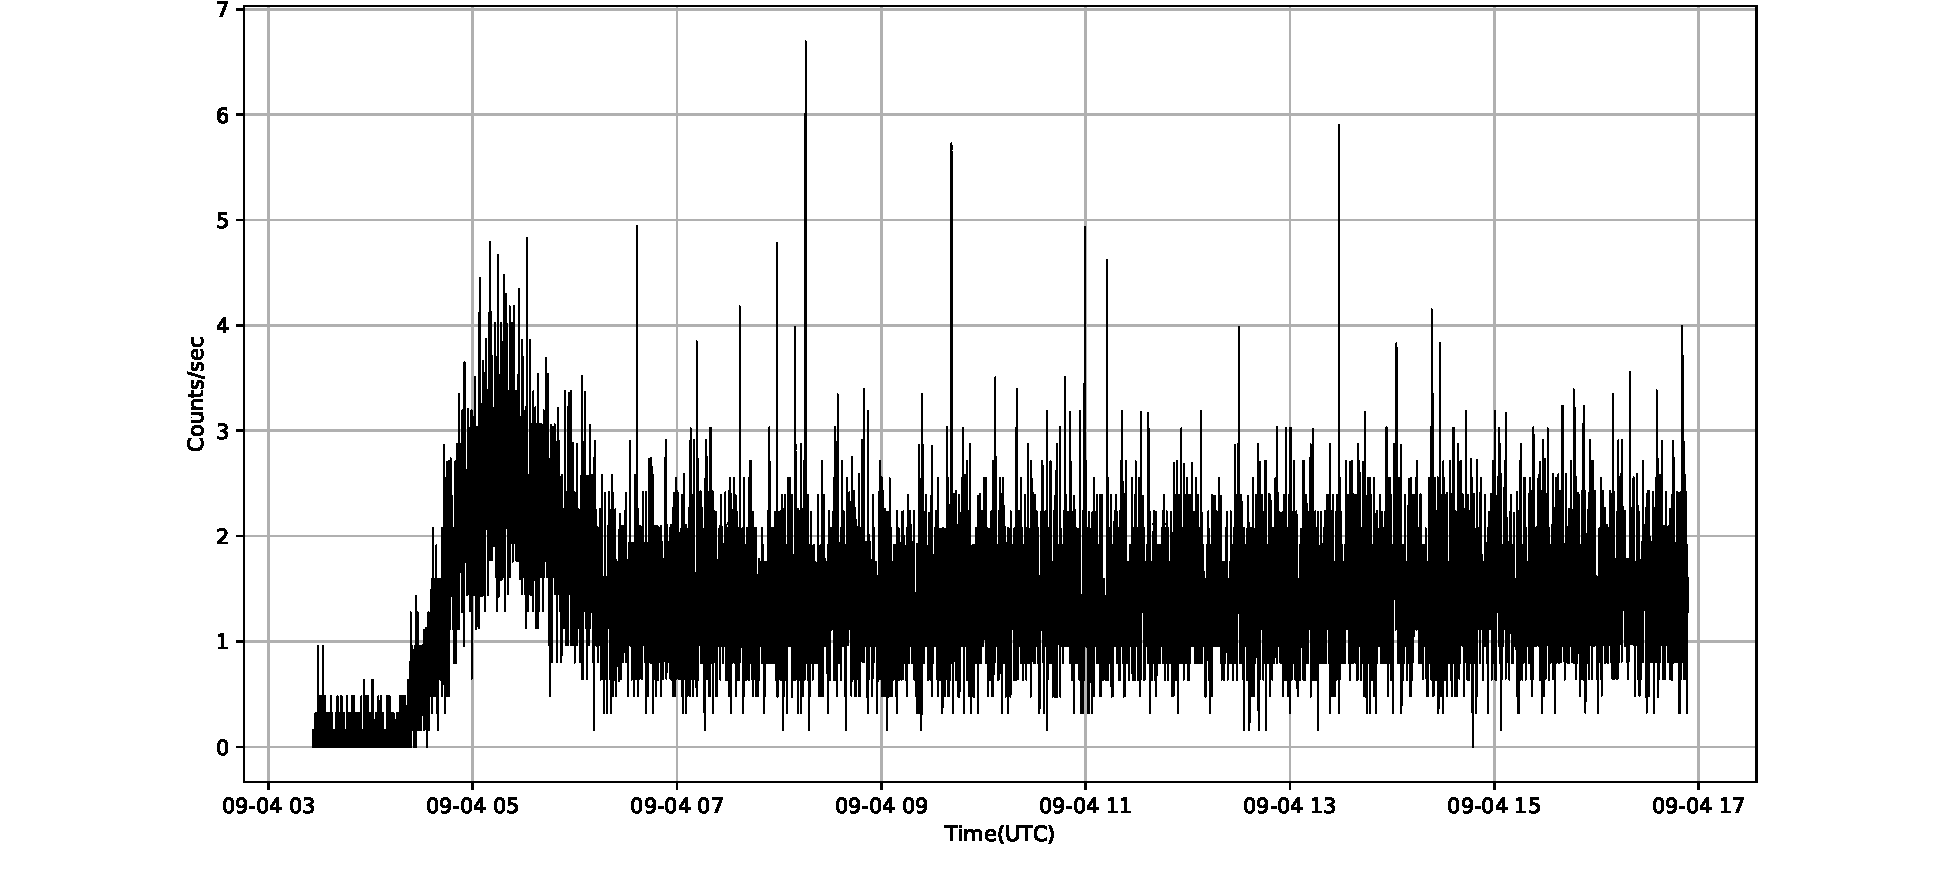
\includegraphics[width=\textwidth]{figures/counts_per_second_2017.pdf}}
\hfill
\subfigure[Counts from data collected during the 2018 flight.]{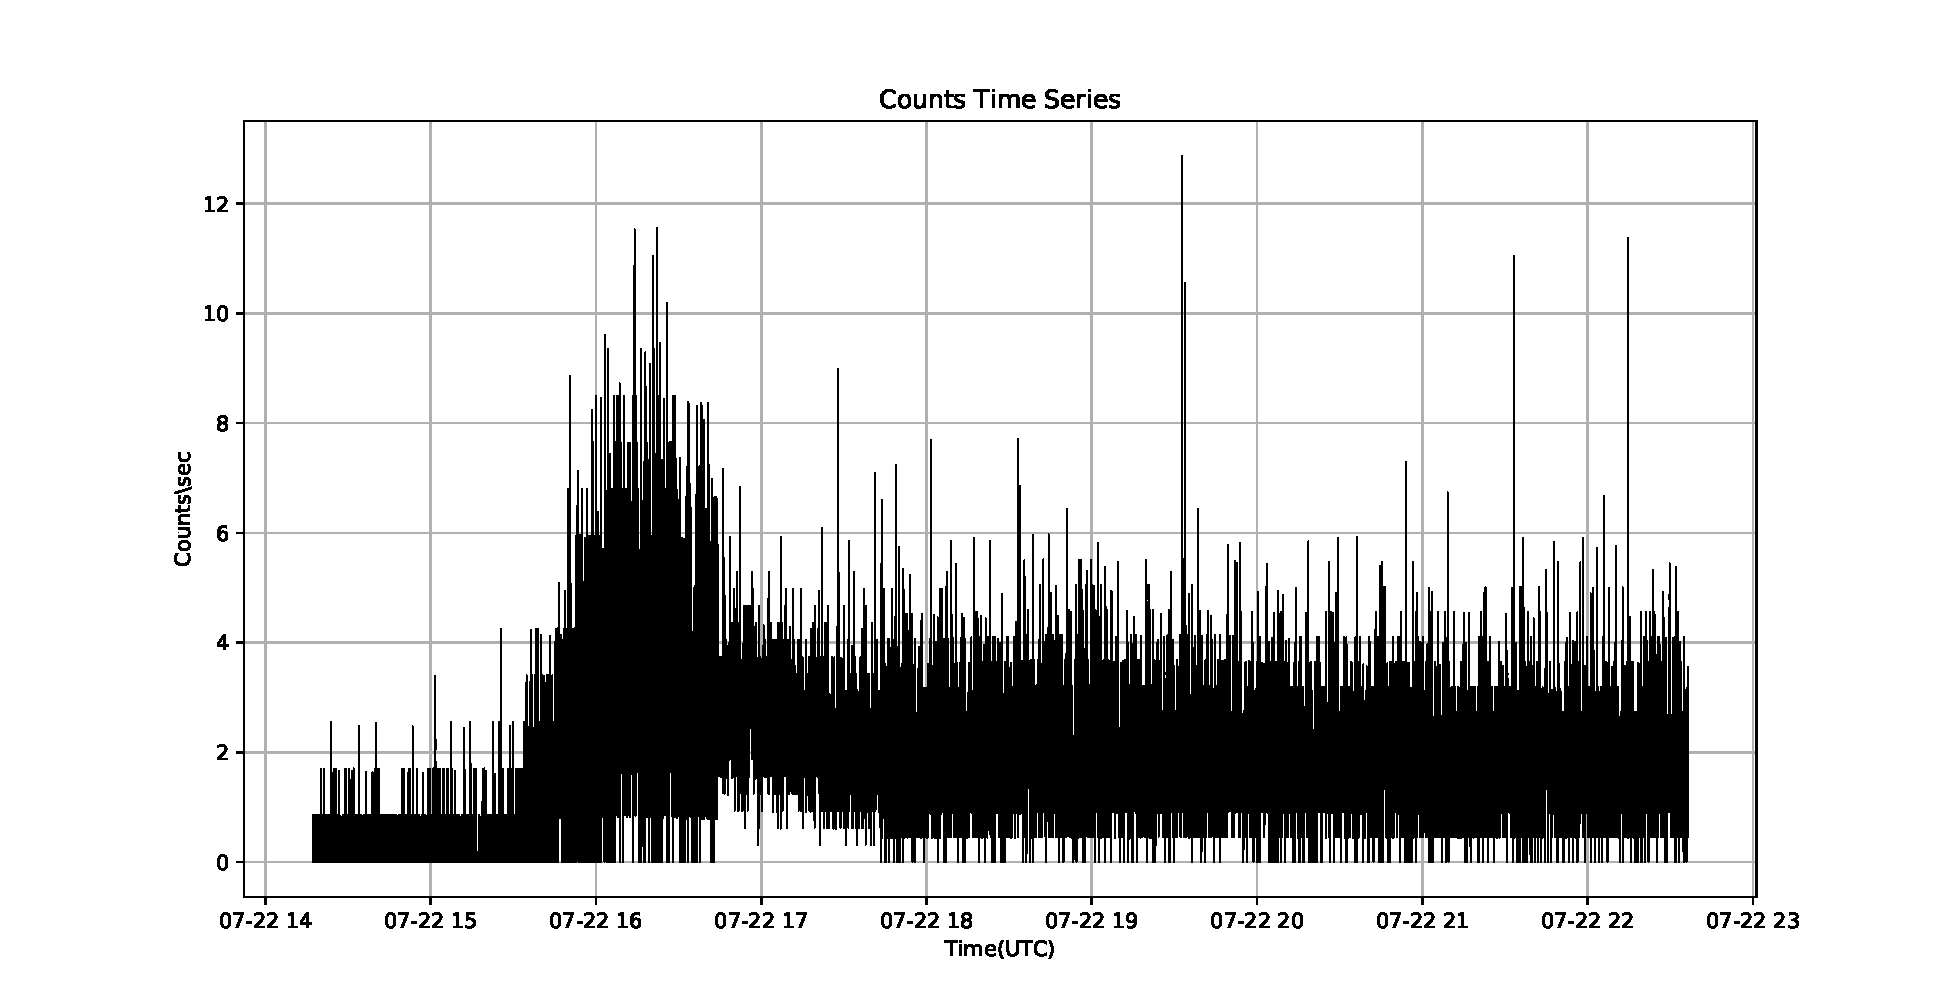
\includegraphics[width=\textwidth]{figures/counts_per_second_2018.pdf}}
\hfill
\caption{Cluster counts data from Flights 2018 and 2017}
\label{counts}
\end{figure}

 %MiniPIX last
\newpage
\subsection{Astrobiology}
\label{sec:Astrobiology-Results}

One goal of this project was to confirm our results from last year. To that end we selected the same 926wF (“AAACTYAAAKGAATTGRCGG”) and 1392R (“ACGGGCGGTGTGTRC***”) primers for the sequencing procedure \cite{SORA}. These primers are designed to amplify 16S RNA from bacterial, archaeal and eukaryotic “universal” samples. The samples were sent to the University of Houston Seq-N-Edit Core and processed using the QIAseq 16S/ITS protocols \cite{QIAseq}. The samples were quantified using a Qubit Fluorometer; the results yielded 28 of the 25-minimum required picograms per micro liter in the experimental sample only. DNA was not detectable in the control samples. The control samples were pooled. Both the pooled control samples and the experimental sample were concentrated using a bead extraction technique. The yield was 248 picograms per micro liter in the experimental sample and 141 picograms per micro liter in the pooled control background sample. Finally, a midpoint quality control check was  performed where it was determined that, while DNA was detectable, the integrity was too low to merit proceeding to the next phase involving several thousand dollars’ worth of materials.  %Astro second

%\input{Results_UV.tex}
%\subsection{Radiation Simulations}
\label{sec:MiniPIX Simulations}

In order to gain an understanding of the data obtained by the MiniPIX, cosmic ray shower simulations will be conducted. The simulations will be of the payload's ascent from Fort Sumner's elevation to float altitude. The software to be used is known as the Dynamic Atmospheric Shower Tracking Interactive Model Application (DYASTIMA) \cite{dyastima}, which utilizes the Geant4 toolkit \cite{geant4}. DYASTIMA provides a wide range of parameters, allowing the user to personalize the conditions for the simulated cosmic ray showers. The parameters to be used are outlined in Table~\ref{tab:dyastima}.

\begin{table}[!h]
  \begin{center}
    \caption{Parameters used for DYASTIMA simulations.} 
    \label{tab:dyastima}
    \bigskip
    \begin{tabular}{|l|l|}
      \hline
      \multicolumn{1}{|l|}{\bf Parameter} &
      \multicolumn{1}{l|}{\bf Value} \\
      \hline
      Planet Radius & \SI{6371.393}{\kilo\meter} \\ \hline
      Simulation Area Width & \SI{800}{\kilo\meter} \\ \hline
      Geometry Model & SPHERE \\ \hline
      Surface Type & NONE \\ \hline
      Air Density Change & 5\% \\ \hline
      Physics List & FTEP\_BERT\_HP \\ \hline
      Range Cut & \SI{1.00}{\meter} \\ \hline
      North Magnetic Field & \SI{22926.6}{\nano\tesla} \\ \hline
      East Magnetic Field & \SI{2993.8}{\nano\tesla} \\ \hline
      Vertical Magnetic Field & \SI{43407.4}{\nano\tesla} \\ \hline
      Surface Pressure & \SI{1024}{\milli\bar} \\ \hline
      Surface Gravity & \SI{9.81}{\meter\per\second\second} \\ \hline
      Spectrum Altitude & \SI{32000}{\meter} \\ \hline
    \end{tabular}
  \end{center}
\end{table}

The values for magnetic field were obtained using a data retrieval tool created by the United States National Oceanic and Atmospheric Administration~\cite{magnetictool} by inputting the exact time and location of the flight's launch. Additionally, DYASTIMA requires the user to input the spectrum list, which requires the particles and various possible energies the particle can possess. 

%74.83 km
 %Simulations results

%Discussion
\input{Discussion_RESU.tex} %RESU first
\subsection{Astrobiology}
\label{sec:Astrobiology Results Discussion}
%We need to go into full detail how changing the payload (removing a pump and half the clean box) may have affected our mission.  This is critical, I believe, since we were only able to see if we captured bacteria, but it limited us to culture it.

Unfortunately, all the information past the Archaea Kingdom classification returned unclassified; which is indicative of missing taxonomic information, at a particular level, retrieved from the National Center for Biotechnology Information (NCBI). For example, if the best match in the RTL Genomic database is classified in NCBI down to Genus, then the RTL Genomic database will label the Species as “Unclassified”. 


There are also instances of “Unknown” and “No Hit” that appear in the results. An “Unknown” classification is an instance where the RTL Genomic database is unable to determine the taxonomic classification at a level with a confidence of at least 0.51 or greater. “No Hit” is assigned for three main reasons. First, when an organism’s sequence is missing from the RTL Genomics database, it can take several months to update the database with new sequencing information from NCBI, European Molecular Biology Laboratory (EMBL) and DNA Data Bank of Japan (DDBL). Additionally, sequences in NCBI, EMBL, and DDBL might be too short or lacking in taxonomic information and are therefore excluded from the RTL Genomic database. Second, an organism’s sequence may not be in any of the major databases, because researchers haven’t finished with updating tasks or the organism may be a new species. The ribosomal RNA synthesis is a great option only if the samples collected are a close enough match to the DNA markers selected to generate a positive hit, otherwise we have no way of knowing if we collected samples representative of a new species. If that were the case, then the only way to test for organisms would be to attempt to culture the samples in conjunction with sequencing. Finally, the sequence may be of low quality and fail to identify as any type of organism. 


There are twenty-nine instances of species classifications with a confidence score of 0.51 or greater in the control sample that are absent in the experimental sample. This may be attributed to the exposure to environmental/float conditions; the control container may have preserved all the bacteria accumulated before the final sealing procedures, but the bacteria did not survive in the experimental sample that was exposed to the upper atmospheric environment. There is also the question of the effects of Archaeal metabolism on its immediate surroundings; there is still a great deal that is yet unknown about Archaeal organisms. The metabolic by-products of any organisms accumulated in the experimental sample may have killed any species accumulated prior to launch.  If the abundance was low enough, these species may not have amplified to a detectable level in the PCR steps.




There are twenty-one instances of species classifications with a confidence score of 0.51 or greater in the experimental sample that are absent in the control sample. It is possible that these organisms were collected around the rim of the tubing outside the payload after it was cut and then pumped into the experimental container once float conditions were reached. However, it is unlikely that all of the organisms were collected this way, since the tubing was drenched in alcohol prior to flight and the potential outside bacteria would have been at risk for hypoxia, hypobaria and other environmental stressors related to reaching float altitude. The uncertainty about these classified species can be addressed in a future design that affords protection to the very outer tubing until float conditions are reached.  


Most convincing is the presence of Archaea in the experimental sample only. Archaea were previously classified as extremophiles only, which leaves room for the possibility that our “Unclassified” Archaea, with a confidence score of at least 0.51, are in fact extremophiles collected from the stratosphere. It would make for a more convincing argument had we replicated our collection and control samples in triplicate; this issue will be addressed in future endeavors. 


While there is room to doubt that every organism absent in the control sample, yet present in the experimental sample, was collected at float altitude, it can be argued with some degree of confidence that it is probable that at least the Archaeal organisms were collected as intended. Culturing the organisms collected in future experiments, in addition to sequencing the 16S rRNA, will provide more concise evidence as to the identity and nature of the organisms collected.


There is much to be learned from living cells that can survive under the float conditions to which our payload was subjected. If our results can be repeated and confirmed, it would also demonstrate that there are more organisms that are able to survive under our payload’s flight conditions than previously documented. 


 %Astro second
\subsection{Radiation}
\label{sec:Radiation Results Discussion}
This is an important discussion of the radiation data.  Discussion discussion discussion. %MiniPIX last
\subsection{MiniPIX Simulations}
\label{sec:MiniPIX Simulations Discussion}
 %Simulations discussion

%Conclusion
\section{Conclusion}
\label{sec:Conclusion}
%%%
%General Guidlines for a conclusion:
%•States whether the purpose was accomplished, and/or hypothesis was supported
%•Backs this up by referring to results
%•Reports final result with uncertainty 
%•Answers any questions posed in the lab manual
%•Addresses any pertinent issues; summarizes discussion, possible sources of error, possible experimental improvements, what has been learned, etc
%
%%%%%this is the conclusion from last year, just for reference.  MAKE SURE TO CITE OUR OWN WORK!!!!!!!!!!!!!!!!
%%RESU
%RESU proved to be efficient and robust.  RESU maintained current below 1.5 $A$ at 30 $V$.  It monitored the environment for the whole duration of the flight flawlessly.  Most sensors operated without a hitch, but a couple of sensors had some issues. The analog temperature sensor used for the electronic pump was found to be reading erroneously, while the magnetometer and orientation sensor recorded noise generated by the electric pump onboard.  Overall, the mission was a testbed for this prototype and allowed us to improve on RESU for future flights.
%
%%Astrobiology
Although DNA was detectable in our samples, we were unable to advance to the next phase in the process of RNA sequencing. We are hopeful that alterations to the DNA extraction protocols will allow for more definitive results in the future. Additionally, a new collection assembly designed to maximize the experimental sample volume is one of the main objectives of next year’s flight. There is much to be learned from living cells that can survive under the float conditions our payload was subjected to at altitude. Genomic, proteomic, and metabolomics comparisons between the high-altitude atmospheric samples and near/at surface samples may yield useful insight into organic radiation shielding and adaptations for survival in extreme conditions. Further missions would help expand on discovering more about these organisms. 

The MiniPIX gathered a wealth of information, with a total of 16,376 frames collected during flight.  The radiation data is still being analyzed. There was a significant increase in particle counts this year, which may be attributed to the addition of the plastic scintillator. The MiniPIX system can be expanded further by the addition of more MiniPIX devices, which would yield a larger volume of data. This year's mission provided a foundation for future flights through the addition of a robust and developed flight computer.  Furthermore, the adjustable MiniPIX system via uplink commands expands the functionality of the payload.
%
%%Radiation
%The particular photodiode we chose for this flight did not have the characteristics to endure the intense exposure of UV light. Nonetheless, the apparatus and ND filters allowed the diodes to operate continuously without saturation under the extreme solar UV irradiance at high altitude. The average maximum irradiance recorded between the three UV photodiodes was \SI{34.8}{\watt\per\meter\squared}. The MiniPIX survived the mission with no issues from the harsh environment in the stratosphere or the crash. The onboard heatsink kept the MiniPIX within working temperatures. Overall, the MiniPIX gathered a wealth of information regarding surrounding radiation, with a peak dosage rate of about \SI{4.2}{\micro\gray\per\hour} at ascent and about \SI{3}{\micro\gray\per\hour} during float.
%
%%Dissemination
%The work performed throughout this project has already begun to be shared around the greater Houston area, starting with presentations at the University of Houston Undergraduate Research Day~\cite{SamURD}~\cite{StevenURD}, expanding to the local Houston community~\citep{StevenSchoolPres}~\cite{Fre}, and even to the APS Texas Section~\cite{SamAPS} in Dallas, TX.  The final results will soon be published in peer reviewed journals, with the articles in preparation now.  Additionally, the team is seeking to patent the different systems and computer systems.  RESU was entered into a competition with MIT for the MIT-Lemelson Award~\cite{MIT} in the "Use it!" catergory. %here it is
 
\newpage
%Appendix
\begin{appendices}
  \section{Collaboration Demographical Information}
\begin{table}[h!]
\centering  
  \begin{tabular}  {ccccccc}
  	\hline
	\hline
    \textbf{Name} &  \textbf{Role} & \textbf{Student Status} & \textbf{Race} & \textbf{Ethnicity} & \textbf{Gender} & \textbf{Disabled}\\
 	\hline
 	Andrew L. Renshaw & Faculty Mentor & Faculty & White & N/A & Male & No\\
 	\hline
 	Samuel A. Garcia Morelos & Project Leader & Post-Bachlor & White & Hispanic & Male & No\\
 	\hline
 	Fre'Etta Brooks & Astrobiology Coordinator & Post-Bachelor & Black & N/A & Female & No\\\hline
 	Steven Oliver & Radiation Coordinator & Post-Bachelor & White & N/A & Male & No\\\hline
 	Reed Masek & Command and Data Handling & Undergrad & White & N/A & Male & No\\\hline
 	Andrew Walker & Lead Programmer & Post-Bachelor & White & Hispanic & Male & No\\\hline
 	Kevin Portillo & Command and Data Handling & Undergrad & White & Hispanic & Male & No \\\hline
	Jimish Patel & Astrobiology & Undergrad & Asian & Indian & Male & No \\ \hline
	Stuart George & MiniPIX Expert & Post-Graduate & White & N/A & Male & No \\ \hline
	Donna Pattison & Faculty Mentor & Faculty & White & N/A & Female & No \\ \hline
	Ian Wilson & Microbiology Expert & Graduate Student & White & N/A & Male & No \\ \hline
	Preethi Gunaratne  & Faculty Advisor & Faculty & Asian & Indian & Female & No \\ \hline
	\end{tabular}	
	\end{table}  

\end{appendices}

\newpage

%References
\newpage

\begin{thebibliography}{9}
\bibitem{SORA}
S.A. Garcia Morelos, F.Brooks, S.Oliver, A.Walker, K.D. Portillo, R.B. Masek, D.Mroczek, D.Pena, J.Juarez, A.Cruz, D. Henandez, S.George, D. Pattison, A.L.Renshaw. \textit{SORA 2017 Mission Webpage}, \url{http://laspace.lsu.edu/hasp/groups/Payload.php?py=2017&pn=10}.

\bibitem{Extremophiles}
  Extremophiles \href{http://www.nytimes.com/2013/02/07/science/living-bacteria-found-deep-under-antarctic-ice-scientists-say.html}{http://www.nytimes.com/2013/02/07/science/living-bacteria-found-deep-\\under-antarctic-ice-scientists-say.html}.

\bibitem{GCRs}
  https://helios.gsfc.nasa.gov/gcr.html

\bibitem{regener}
  Regener E. \& Pfotzer G., \textit{Vertical Intensity of Cosmic Rays by Threefold Coincidences in the Stratosphere.}, Nature 136, 718-719, (1935). 

%\bibitem{NeutronDensity}
 % Haymes, R. C., Reidy, W. P., \& Korff, S. A. (1962). The Cosmic Ray Neutron Density at High Altitudes. Journal of the Physical Society of Japan, 17, 115-117.

\bibitem{SolarCycle}
  Hathaway, D. H. (2015). The Solar Cycle. Living Reviews, 12. doi:10.1007/lrsp-2015-4
  
\bibitem{Frank}
  Schröder, F. G. (2017). Radio detection of cosmic-ray air showers and high-energy neutrinos. Progress in Particle and Nuclear Physics, 93, 1-68. doi:10.1016/j.ppnp.2016.12.002
    
\bibitem{BoronScintillator}
  EJ-254 Boron Loaded Plastic Scintillator \url{https://eljentechnology.com/images/products/data_sheets/EJ-254.pdf}.

\bibitem{Pawelczak}
  Pawełczak, I., Glenn, A., Martinez, H., Carman, M., Zaitseva, N., \& Payne, S. (2014). Boron-loaded plastic scintillator with neutron-$\gamma$ pulse shape discrimination capability. Nuclear Instruments and Methods in Physics Research Section A: Accelerators, Spectrometers, Detectors and Associated Equipment, 751, 62-69. doi:10.1016/j.nima.2014.03.027

\bibitem{cleanbox}
  Clean box material \url{https://www.mcmaster.com/\#uhmw-polyethylene/=1aijn1p}.

\bibitem{silicon_sensor}
  MiniPIX - Miniaturized Portable USB Photon Counting Camera. (n.d.). Retrieved February 02, 2017, from \url{http://advacam.com/camera/minipix}.

\bibitem{timepix}
  Timepix chip at \url{https://medipix.web.cern.ch/technology-chip/timepix3-chip}

\bibitem{medipix}
  Medipix collaboration at \url{https://medipix.web.cern.ch/}.

\bibitem{Uher}
  Uher, J., Frojdh, C., Holy, T., Jakubek, J., Petersson, S., Pospisif, S., . . . Stekl, I. (2007). Silicon Detectors for Neutron Imaging. AIP Conference Proceedings. doi:10.1063/1.2825756
  
\bibitem{Seq-N-Edit Core}
  UH Seq-N-Edit Core at \url{http://seqnedit.nsm.uh.edu/}.
  
\bibitem{QIAseq}
  QIAseq Protocols at \url{https://www.qiagen.com/us/resources/resourcedetail?id=07fa061e-c9e8-44b9-9b09-6af351e632cd&lang=en}.  

\bibitem{PowerWaterKit}
  PowerWater Kit Protocols at \url{https://www.qiagen.com/us/resources/resourcedetail?id=bb731482-874b-4241-8cf4-c15054e3a4bf&lang=en}.  
  
\bibitem{stuartthesis}
  George, S., \textit{Dosimetric Applications of Hybrid Pixel Detectors}, University of Wollongong, Australia, 2015.

\bibitem{stuartalgo}
  Reprinted from \textit{Dosimetric Applications of Hybrid Pixel Detectors} by Stuart George, 2015, Mixed Field Measurements and Cluster Formation with Timepix,52.

%\bibitem{LSU}
%  Christner, B., Alleman, M., Bryan, N., Burke, S., Guzik, T.G., Granger, D., King, G. (2013) \textit{LSU HASP2013 PDF. Baton Rouge: Louisiana Space Consortium}.

%\bibitem{Solidworks}
%  SolidWorks 3D CAD software \url{http://www.solidworks.com/}.
  
%\bibitem{COMSOL}
%  COMSOL Multiphysics Simulation software \url{http://www.comsol.com}.

%\bibitem{canales}
% Canales D. C. and Ehteshami A., \textit{An attempt to sample atmospheric bacteria}, Houston, TX, 2015, January 11.

%\bibitem{bexus}
%Urbar, J., Scheirich, J., Jakubek, J., 2011. Medipix/Timepix cosmic ray tracking on BEXUS stratospheric balloonflights. Nucl. Instrum. Methods A 633, S206-209.
	
%\bibitem{uv_irradiance}
%  Calculating the UV Index. (2016, October 14). Retrieved June 03, 2017, from \url{https://www.epa.gov/sunsafety/calculating-uv-index-0}.

%\bibitem{UVonDNA}
%  Cockell CS, Horneck G., \textit{The history of the UV radiation climate of the earth--theoretical and space-based observations.}, Photochem Photobiol. 73(4):447-51 (2001).

%\bibitem{valve}
%  Valve data sheet \url{http://www.generant.com/Literature/Series\%20VRV\%20Product\%20Literature.pdf}.

%\bibitem{Thor Labs} 
%  Thor Labs, \textit{Unmounted UV Fused Silica Reflective ND Filters}. Retrieved August, 18, 2017, from \url{https://www.thorlabs.com/newgrouppage9.cfm?objectgroup_id=6106}.

%\bibitem{RTL}
%  RTL Genomics at \url{http://rtlgenomics.com/}.

%\bibitem{lemon}
%PCR Method at \url{http://www.journal-of-hepatology.eu/article/S0168-8278(17)32278-X/fulltext}.
	
%\bibitem{illumina}
%  Illumina, Inc. San Diego, California at \url{https://www.illumina.com/}

%\bibitem{Microbial rRNA sequencing}
%Microbial rRNA sequencing \url{http://pubs.rsc.org/En/content/articlehtml/2017/em/c6em00413j}.

%\bibitem{mpdatasheet}
%  ADVACAM, \textit{MINIPIX Version 1.0 Datasheet}, Retrieved from \url{http://www.widepix.cz/files/datasheets/MiniPIX\%20v1.0\%20Datasheet.pdf}.

%\bibitem{numpy} 
%  Numpy scientific computing library at \url{http://www.numpy.org/}.

%\bibitem{spaceballoonnetwork}
%  Space weather archives \url{http://spaceweather.com/archive.php?view=1&day=12&month=10&year=2016}.

%\bibitem{dyastima}
%  Paschalis, P. et al., \textit{Geant4 software application for the simulation of cosmic ray showers in the Earth? atmosphere. New Astronomy} {\bf 33} (2014):26.

%\bibitem{geant4}
%  Geant4 simulation toolkit at \url{http://geant4.cern.ch/}.

\bibitem{mpjakubek}
  Jan Jakubek, \textit{Precise energy calibration of pixel detector working in time-over-threshold mode} Institute of Experimental and Applied Physics, Czech Technical University in Prague, Czech Republic, 2011.

%\bibitem{magnetictool}
%  United States National Oceanic and Atmospheric Administration, \textit{Magnetic Field Calculators} [Data sets], Retrieved from \url{https://www.ngdc.noaa.gov/geomag-web/#igrfwmm}.

%\bibitem{gorman}
%	Gorman, J. (2013, February 06). \textit{Scientists Find Life in the Cold and Dark Under Antarctic Ice.} Retrieved September 15, 2016, from Scientists Find Life in the Cold and Dark Under Antarctic Ice.
	 
%\bibitem{pumpsource}
%  \url{http://www.knfusa.com/?type=5600&amp;file=2079}.

%\bibitem{Horneck}
%  Horneck, G. 1993. The Biostack concept and its application in space and at accelerators: studies in Bacillus subtilis spores, p. 99-115. In C. E. Swenberg, G. Horneck, and E. G. Stassinopoulos (ed.), \textit{Biological effects and physics of solar and galactic cosmic radiation}[PDF], part A. Plenum Press, New York, NY. accessed 10/24/16  

%\bibitem{Horneck} 
%  Horneck, G. 2007. \textit{Space radiation biology}[PDF], p. 243-273. In E. Brinckmann (ed.), Biology in space and life on Earth. Wiley-VCH, Weinheim, Germany. Accessed 10/26/16

%\bibitem{Horneck}
%  Horneck, G., C. Baumstark-Khan, and G. Reitz. 2002. \textit{ Space microbiology: effects of ionizing radiation on microorganisms in space}[PDF], p. 2988-2996. In G. Bitton (ed.), The encyclopedia of environmental microbiology. John Wiley \& Sons, New York, NY. Accessed 10/30/16

%\bibitem{Horneck}
%  Horneck, G., C. Baumstark-Khan, and R. Facius. 2006. \textit{Radiation biology}[PDF], p. 292-335. In G. Cl?ment and K. Slenzka (ed.), Fundamentals of space biology. Kluwer Academic Publishers/Springer, Dordrecht, The Netherlands. accessed 11/4/16

%\bibitem{Kiefer}
%Kiefer, J., K. Schenk-Meuser, and M. Kost. 1996. \textit{Radiation biology}[PDF], p. 300-367. In D. Moore, P. Bie, and H. Oser (ed.), Biological and medical research in space. Springer, Berlin, Germany. accessed 11/9/16
 
%\bibitem{SamURD}
%	Alfonso Garcia Morelos, S. (2016, October 13).
%	\textit{A Novel Microbe Trap.}
%	Presentation at UH Undergraduate Research Day. \url{http://www.uh.edu/honors/undergraduate-research/}
		
%\bibitem{StevenURD}

%\bibitem{FreEttaWomensConference}

%\bibitem{StevenSchoolPres}

%\bibitem{StevenURD}
%  Oliver, S. J. (2017, October 12). 
%  \textit{Stratospheric Organism and Radiation Analyzer}
%  Presentation at UH Undergraduate Research Day. Retrieved October 12, 2017, from \url{http://www.uh.edu/honors/undergraduate-research/events/urday2017/}

%\bibitem{StevenSchoolPres}
%  Oliver, S. J. (2017, November 4). 
%  \textit{STEM Life at UH}
%  Presentation at UH Gathering of the Eagles STEM Symposium. \url{https://www.uh.edu/news-events/stories/2016/November/110416EaglesSTEM.php}

%\bibitem{Fre}
%  Brooks, F. (2017, January 14).
%  \textit{Stratospheric Organism and Radiation Analyzer}
%  Presentation at Rice University, APS Conferences for Undergraduate Women in Physics (CUiP). \url{http://www.google.com/url?q=http%3A%2F%2Fwww.aps.org%2Fprograms%2Fwomen%2Fworkshops%2Fcuwip.cfm&sa=D&sntz=1&usg=AFQjCNE5pImV-SVrb87CvgAa9RSfeCrYXg}  
  
%  \bibitem{SamAPS}
%	Alfonso Garcia Morelos, S. (2017, October 20).
%	\textit{Stratospheric Organism and Radiation Analyzer}
%	Retrieved October 20, 2017, from \textit{Bulletin of the American Physical Society}. \url{https://meetings.aps.org/Meeting/TSF17/Session/E5.3}
	
%\bibitem{MIT}
%  MIT-Lemelson Award 2018.
%  \url{https://lemelson.mit.edu/}  

\end{thebibliography}
%Bibliography file

%
\clearpage
%\bibliographystyle{SORA}
%\bibliography{SORA}
\end{document}
